\newcommand{\anonsection}[1]{\section*{#1}\addcontentsline{toc}{section}{#1}}
\newcommand{\anonsubsection}[1]{\subsection*{#1}\addcontentsline{toc}{subsection}{#1}}
\newcommand{\anonsubsubsection}[1]{\subsubsection*{#1}\addcontentsline{toc}{subsubsection}{#1}}

\documentclass[10pt]{article}
\usepackage{a4wide}
\usepackage[utf8]{inputenc}
\usepackage[russian]{babel}
\usepackage{graphicx}
\usepackage{amsmath}
\usepackage{amsfonts}
\usepackage{caption}
\usepackage{subfig}
\usepackage[left=3cm,right=3cm, top=3cm,bottom=3cm,bindingoffset=0cm]{geometry}
\usepackage{hyperref}
\usepackage{amsthm}

\newtheorem{theorem}{Теорема}
\newtheorem{definition}{Определение}
\newtheorem{statement}{Утверждение}


\numberwithin{equation}{section}

\begin{document}

\thispagestyle{empty}

\begin{center}
\ \vspace{-3cm}


\includegraphics[width=0.5\textwidth]{msu.png}\\
{\scshape Московский государственный университет имени М.~В.~Ломоносова}\\
Факультет вычислительной математики и кибернетики\\
Кафедра системного анализа

\vfill

{\LARGE Курсовая работа. }

\vspace{1cm}

{\Huge\bfseries Динамические системы и модели биологии.}
\end{center}

\vspace{1cm}

\begin{flushright}
  \large
  \textit{Студент 315 группы}\\
  Е.\,В.~Гуров

  \vspace{5mm}

  \textit{Научный руководитель}\\
  Д.\,А.~Алимов
\end{flushright}

\vfill

\begin{center}
Москва, 2021
\end{center}
\newpage

\tableofcontents
\newpage

\anonsection{Динамические системы с дискретным временем}
\anonsubsection{Постановка задачи}
\setcounter{section}{1}

Даны две динамические системы с дискретным временем:
\begin{enumerate}
	\item Одномерная:
	\begin{equation} \label{first_system}
		u_{t+1} = ru_te^{-\frac{r}{2}u_t^2} \ , \ u_t > 0 \  , \ \forall t \in \mathbb{N}.
	\end{equation}
	\item Двумерная:
	\begin{equation} \label{second_system}
		u_{t+1} = ru_te^{-\frac{r}{2}u_{t-1}^2} \ , \ u_t > 0 \  , \ \forall t \in \mathbb{N}.
	\end{equation}
\end{enumerate}

\begin{itemize}
	\item Найти неподвижные точки и исследовать их устойчивость.
	\item Доказать, что имеется цикл длины 2.
	\item Найти циклы длины 3 и построить бифуркационную диаграмму в зависимости от значения параметра \( (r > 0) \).
	\item Построить зависимость показателя Ляпунова от значения парметра \( (r > 0) \).
	\item Для системы с запаздыванием построить бифуркационную диаграмму, построить инвариантную кривую в случае существования бифуркации Неймарка-Сакера.
\end{itemize}

\anonsubsection{Исследование одношаговой системы}
Начнем с того, что исследуем систему (\ref{first_system}) на наличие и характер неподвижных точек.
\anonsubsubsection{Неподвижные точки}
Для начала дадим определение неподвижной точки.
\begin{definition}
	Точка \(u^* \in \mathbb{R} \) называется неподвижной точкой системы \( u_{t+1} = f(u_t) \ , \ u_t \in \mathbb{R} \ , \ f : \mathbb{R} \to \mathbb{R}\),  если \( u^* = f(u^*) \).
\end{definition}

\noindent Таким образом для нахождения неподвижных точек нужно решить уравнение:
\[ f(u,r) = u \ , \ r > 0. \]

\noindent Учитывая, что \( f(u,r) = rue^{-\frac{r}{2}u^2}\), получим:
\[ rue^{-\frac{r}{2}u^2} = u \ , \ r > 0. \]
Решая это уравнение, с учетом ограничений на \( u \) находим две неподвижные точки: \( u_1^* = 0, u_2^* = \sqrt{\frac{2\ln{r}}{r}} \). Первая из них существует всегда, а вторая возникает при \( r > 1\).

\anonsubsubsection{Исследование характера неподвижных точек}
Для начала введем необходимые определения и утверждения.

\begin{definition}[Определение устойчивости точки по Ляпунову]
	Неподвижная точка \(u^*\) динамической системы \( u_{t+1} = f(u_t) \ , \ u_t \in \mathbb{R} \ , \ f : \mathbb{R} \to \mathbb{R} \) называется устойчивой по Ляпунову, если для любого \( \varepsilon > 0 \) существует \( \delta > 0 \) такое, что для любого \( u_0 : \|u_0 - u^*\| < \delta \) выполняется неравенство  \( \|u_t - u^*\| < \varepsilon \) для всех t > 0. В противном случае точка называется неустойчивой. 
\end{definition}

\begin{definition}
	Если \( u^* \) --- устойчивая по Ляпунову неподвижная точка системы \( u_{t+1} = f(u_t) \ , \ u_t \in \mathbb{R} \ , \ f : \mathbb{R} \to \mathbb{R} \)
и , кроме того, \( \lim\limits_{t \to \infty} f(u_t) = u^* \), то \( u^* \) называется асимптотически устойчивой по Ляпунову.
\end{definition}

\begin{statement}
	Пусть \( u^* \) --- неподвижная точка системы \( u_{t+1} = f(u_t) \ , \ u_t \in \mathbb{R} \ , \ f : \mathbb{R} \to \mathbb{R} \), и пусть \( f \) обратима в малой окрестности \( u^* \). Тогда \( u^* \) асимптотически устойчива, если \( |f_u'(u^*)| < 1 \), и неустойчива, если \( |f_u'(u^*)| > 1 \).
\end{statement} 
\begin{proof}
	Доказательство этого утверждения можно найти в \cite{1} на странице 83.
\end{proof}

\noindent Таким образом, для выяснения характера неподвижных точек данной системы исследуем:
\[ |f_u'(u^*, r)|  = |re^{-\frac{r}{2}(u^*)^2} - r^2(u^*)^2 e^{-\frac{r}{2}(u^*)^2}| = |re^{-\frac{r}{2}(u^*)^2}(1 - r(u^*)^2) |. \] 

\begin{enumerate}
	\item \( f_u'(u_1^*, r) = r \). Тогда при \( 0 < r < 1 \) точка \( u_1^* \) устойчива, при \( r > 1 \) неустойчива.
	\item \( f_u'(u_2^*, r) = 1 - 2\ln{r} \).
\end{enumerate}
	\[ |1 - 2\ln{r}| < 1 \iff \begin{cases} 1 - 2 \ln{r} < 1 \\ 1 - 2 \ln{r} > -1 \end{cases}  \iff \begin{cases} \ln{r} > 0 \\ \ln{r} < 1 \end{cases} \iff  \begin{cases} r > 1 \\ r < e \end{cases}\]
\noindent То есть точка \( u_2^* \) устойчива при \( r \in (1; e) \) и неусточива при \( r > e \).

\begin{figure}[h]
    \centering
    \subfloat[\centering Траектория системы при r = 0.8(точка \( u_1^* \) ассимптотически устойчива)]
{{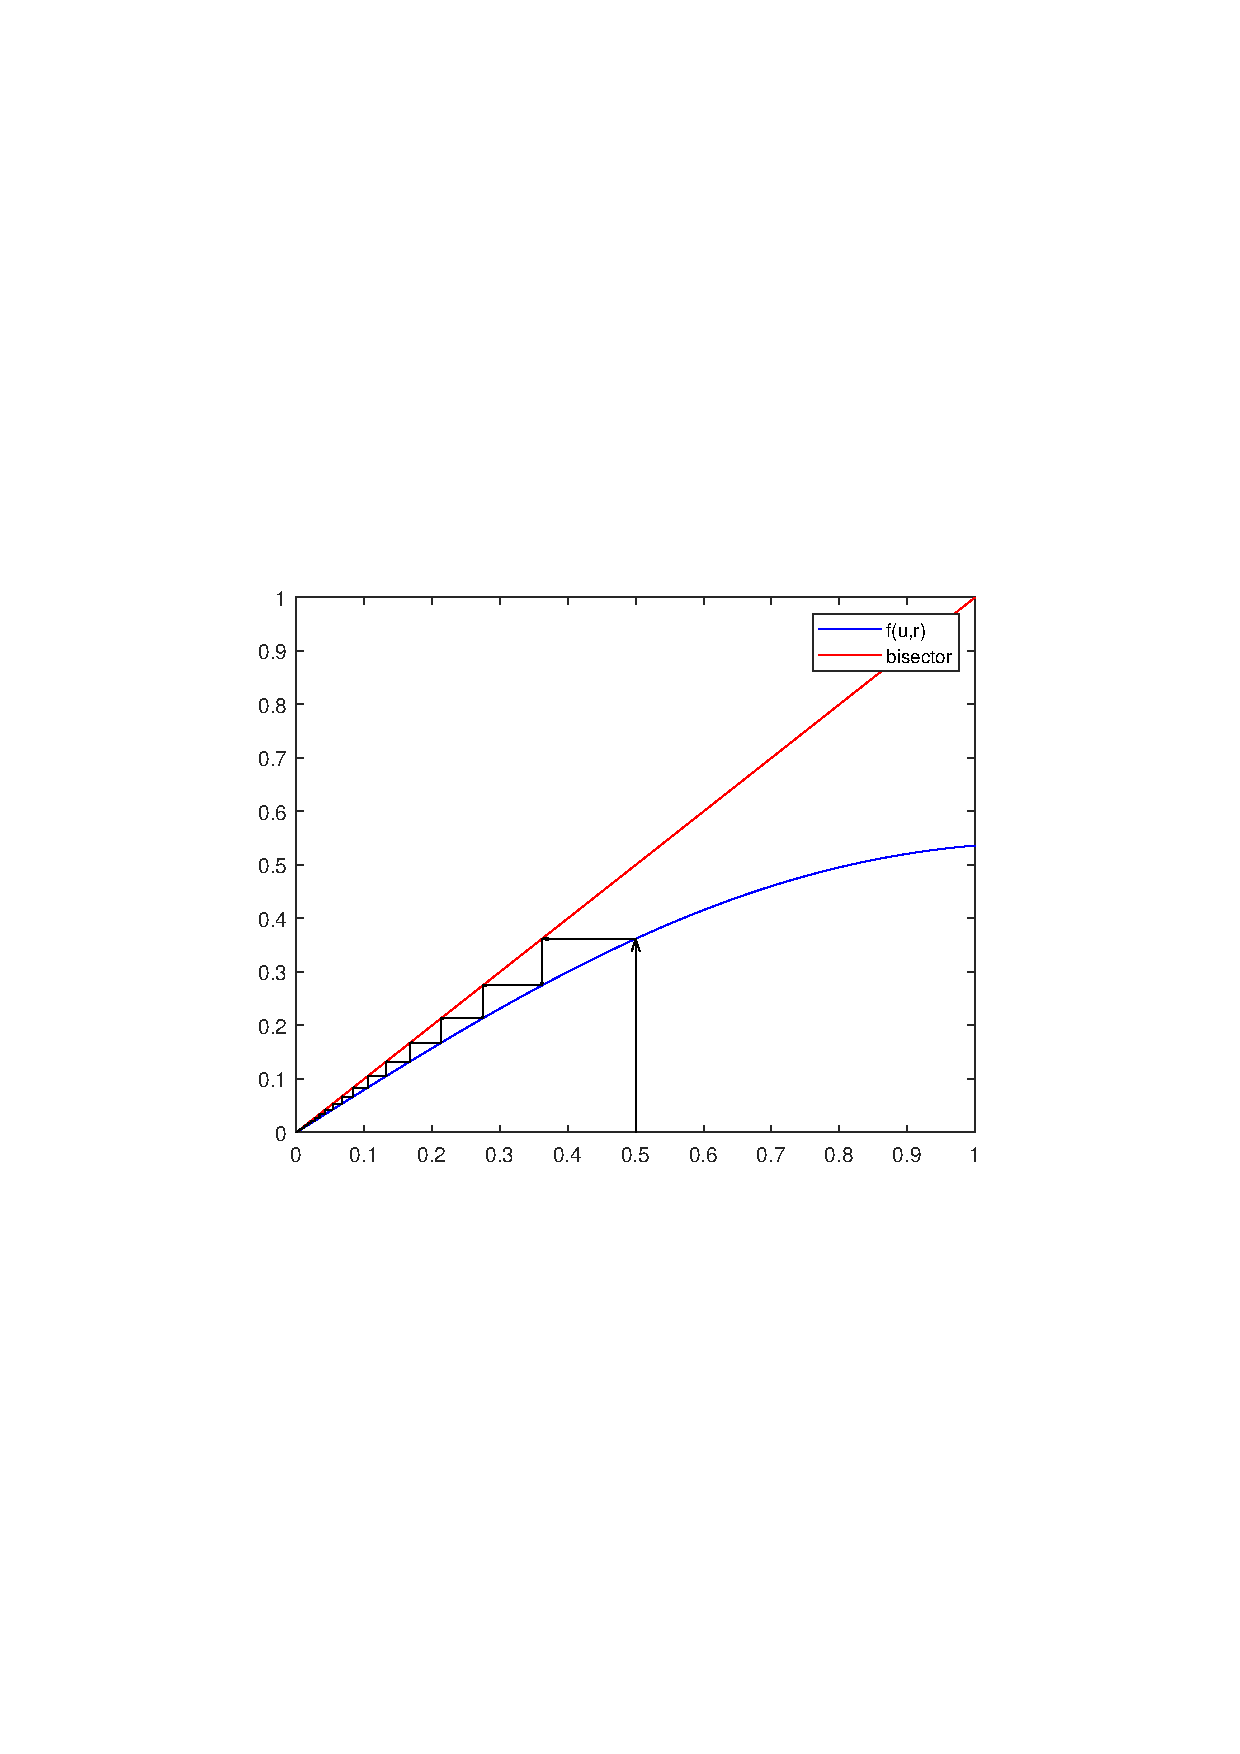
\includegraphics[width=7cm]{r_0.8.pdf} }}
    \qquad
    \subfloat[\centering Траектория системы при r = 2.5(точка \( u_1^* \) неустойчива, точка \( u_2^* \) ассимптотически устойчива)]{{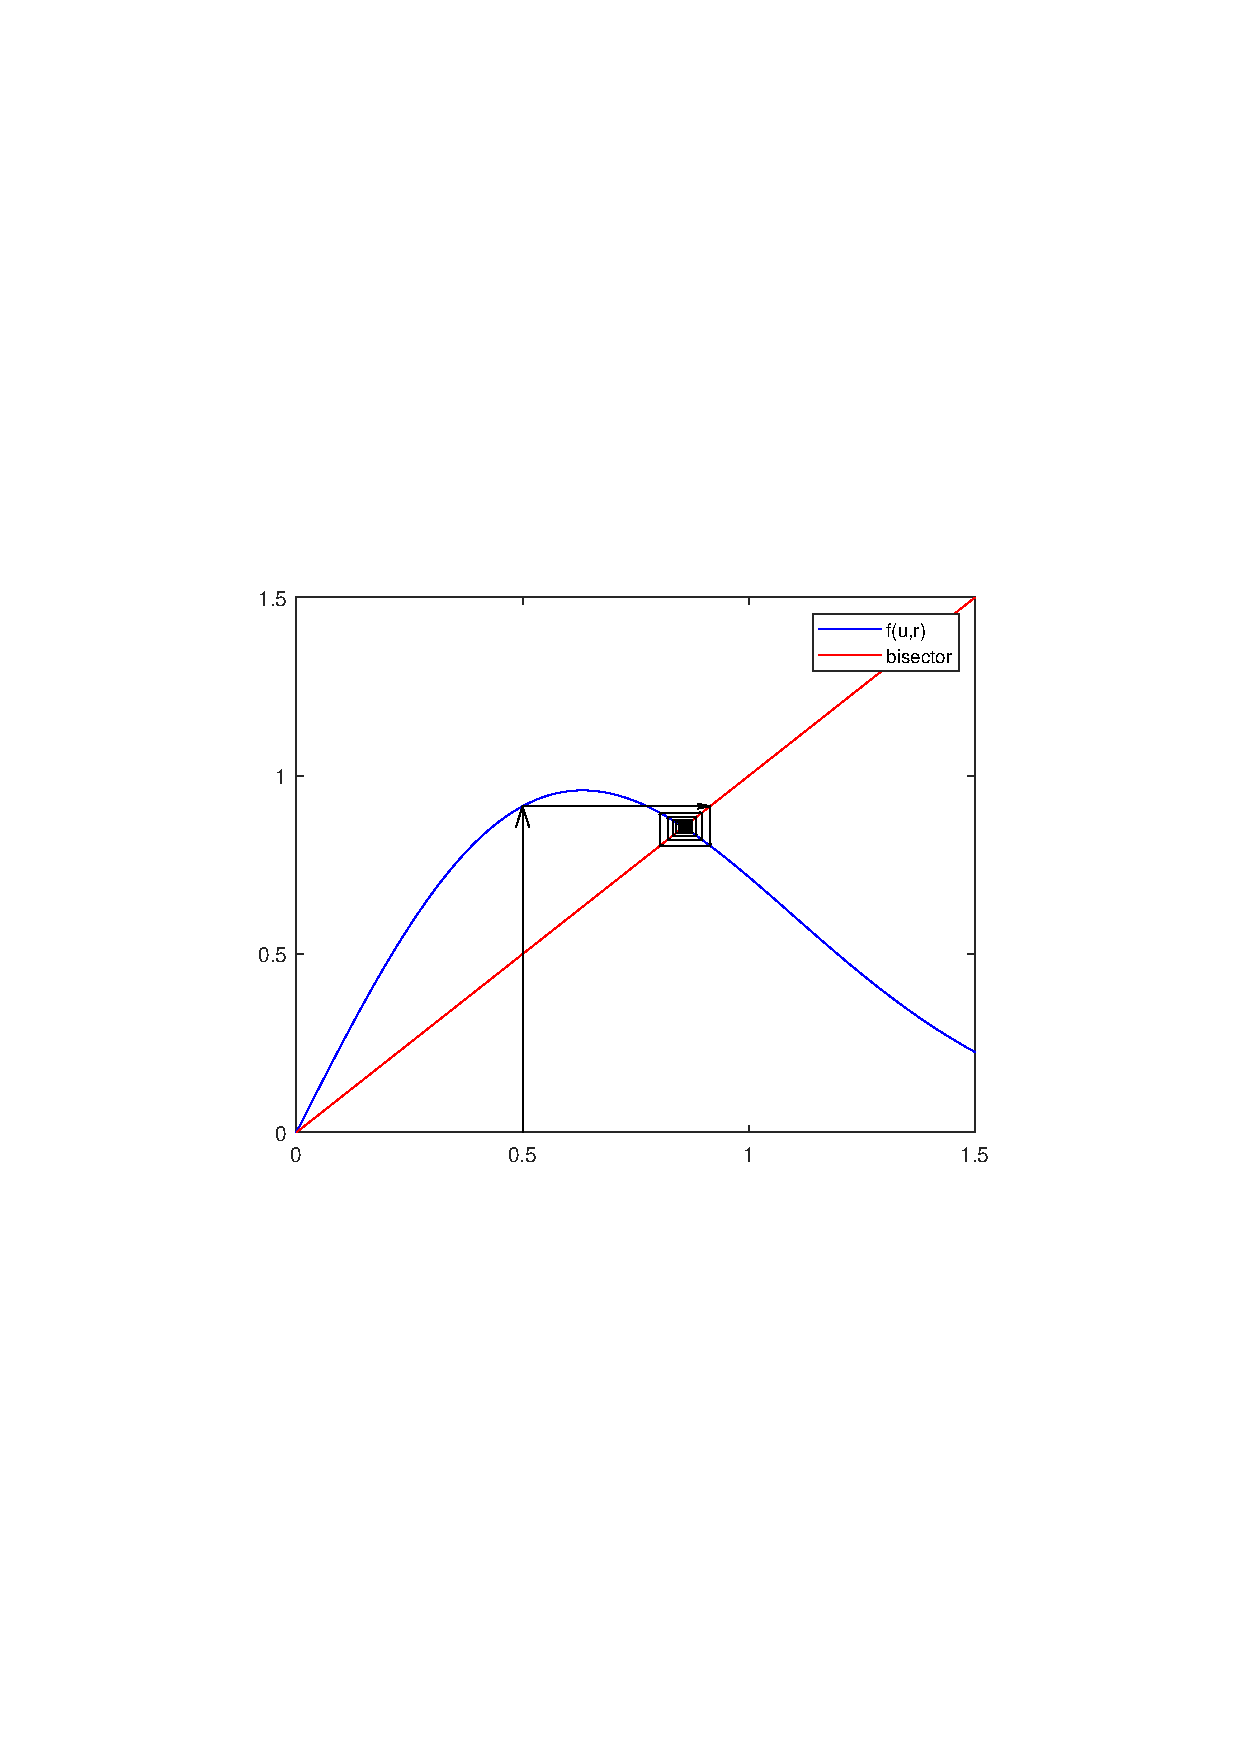
\includegraphics[width=7cm]{r_2.5.pdf} }}
    \caption{Устойчивость точек при разных значениях параметра \( r \).}
\end{figure}

\anonsubsubsection{Исследование системы на наличие циклов. Построение бифуркационной диаграммы.}
Рассмотрим дискретную динамическую систему, определяемую отображением \( f \):
\begin{equation}\label{discr_system}
	u \mapsto f(u) = f(u,r) \ , \ u \in U \subset \mathbb{R} \ , \ r \in \mathbb{R} \ , \ f: U \to U .
\end{equation}

\begin{definition}
	Множество всевозможных состояний \( u_t \) называется пространством состояний (или фазовым пространством) системы (\ref{discr_system}).
\end{definition}

\begin{definition}
	Множество точек \( u_t , t = 0, 1, \dots \), где \(u_t = f(u_{t-1})\), называется траекторией (или орбитой) системы (\ref{discr_system}), порожденной отображением \( f \).
\end{definition}

\begin{definition}
	Динамическая система \( u \mapsto f(u) \) называется топологически эквивалентной в области \( U \subset \mathbb{R} \) динамической системе \( v \mapsto g(v) \) в области \( V \subset \mathbb{R} \), если существует гомеоморфизм \( h : \mathbb{R} \to \mathbb{R}  \ , \ h(U) = V\), отображающий орбиты первой системы в \( U \) на орбиты второй системы в \( V \), сохраняя ориентацию во времени.
\end{definition}

\begin{definition}
	Появление топологически неэквивалентных фазовых портретов при изменении параметров системы называется бифуркацией.
\end{definition}

\begin{definition}
	Бифуркационной диаграммой динамической системы называется разбиение пространства праметров на максимальные свзяные подможества, которые определяются соотношениями топологической эквивалентности и рассматриваются вместе с фазовыми портретами для каждого элемента разбиения.
\end{definition}

\begin{definition}
	Циклом длины \( k \) дискретной динамической системы 
	\[ u_{t+1} = f(u_t) \ , \ u_t \in \mathbb{R},\]
	называется множество различных точек \( u_1, u_2, \dots, u_k \) таких, что 
	\[u_2 = f(u_1), \dots, u_k = f(u_{k-1}), u_1 = f(u_k).\]
\end{definition}

Построим бифуркационную диаграмму для системы (\ref{first_system}). С помощью нее можно определить наличие устойчивых циклов и их длину при разных занчениях параметра \( r \). Построим график, на оси абсцисс которого расположим значения параметра \( r \), а на оси ординат точки, в которых система находится последовательно \( m \) раз после выполнения \( n \) итераций.(в случае наличия предельных циклов эти \( m \) состояний будут приближенно совпадать). Для этого выберем произвольную начальную точку \( u_0 \), и для каждого значения \( r \) на некоторой сетке проведем n итераций. После чего проведем еще \( m \) итераций, на которых будем отмечать точки в которых оказывается система. 

\begin{figure}[h]
	\center{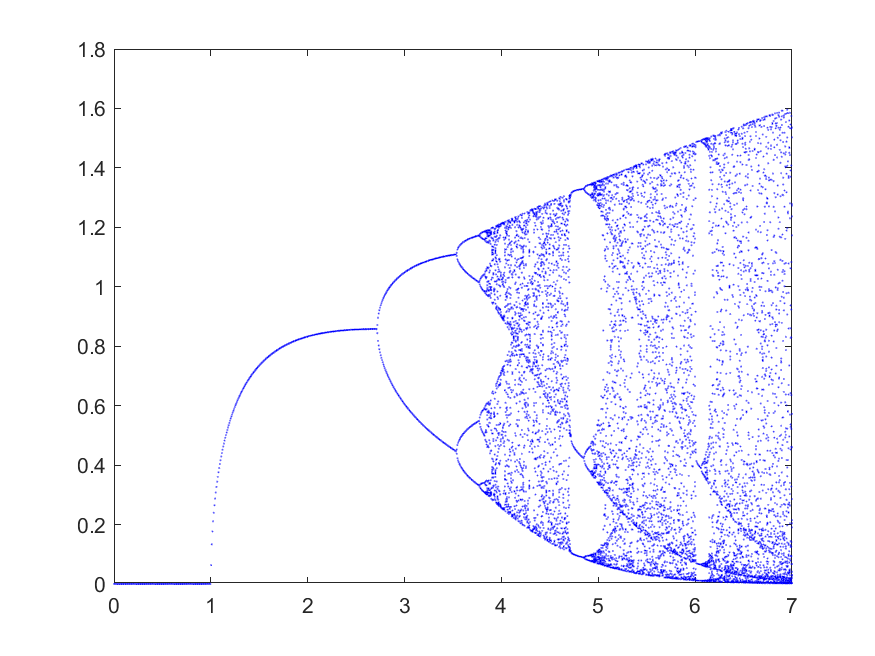
\includegraphics[scale = 0.8]{bifurcation_diagram.pdf}}
	\caption{Бифуркационная диаграмма для системы (\ref{first_system}). n = 1000, m  = 20.}
\end{figure}

\begin{definition}
	Упорядочиванием множества натуральных чисел по Шарковскому назовем упорядочивание натуральных чисел по следующему порядку:
	\[ 3 \succ 5 \succ 7 \succ \dots \succ \]
	\[\succ 2\cdot 3 \succ 2\cdot 5 \succ 2 \cdot 7 \succ \dots \succ \]
	\[\succ 2^2\cdot 3 \succ 2^2\cdot 5 \succ 2^2 \cdot 7 \succ \dots \succ \]
	\[\succ 2^3\cdot 3 \succ 2^3\cdot 5 \succ 2^3 \cdot 7 \succ \dots \succ \]	
	\[\succ \dots \succ \]
	\[\succ 2^3 \succ 2^2 \succ 2 \succ 1.\]
\end{definition} 

\begin{theorem}[А.Н. Шарковский]
	Пусть \( f : \mathbb{R} \to \mathbb{R} \) --- непрерывное отображение, и пусть \( f \) имеет цикл длины \( k \). Тогда система имеет цикл длины \( m \) для всех таких \( m \), что \( k \succ m \) в смысле порядка по Шарковскому. 
\end{theorem}
\begin{proof}
	Доказательство этого утверждения можно найти в \cite{1} на странице 89.
\end{proof}
	

В силу определения цикла, каждая из \( k \) точек цикла является неподвижной точкой \( k \)-ой интерации отображения
\[ f^k(u) = f(f(\dots f(u))) = \underbrace{f \circ \dots \circ f}_k. \]
Таким образом, для точного нахождения параметров, при которых возможны циклы длины три, можно решить систему:
\[ \begin{cases} f^3(u,r) = u \\ (f^3(u,r))_u' = 1, \end{cases}\]
где \( f^3 = f \circ f \circ f . \)\\
Таким образом находим значение параметра \( r \), при котором появляется устойчивый цикл длины три и точки этого цикла:
\[ r = 4.717, u_1 = 0.107, u_2 = 0.492, u_3 = 1.310 \]

\begin{figure}[h]
    \centering
    \subfloat[\centering График \( f^3 \) с тремя точками касания биссектрисы первого координатного угла.]{{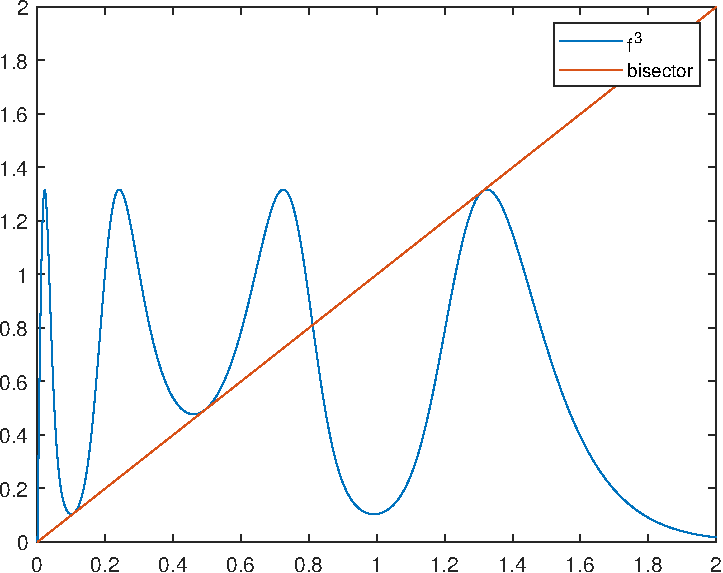
\includegraphics[width=7cm]{f3.pdf} }}
    \qquad
    \subfloat[\centering Траектория системы, соответствующая устойчивому чиклу длины три.]{{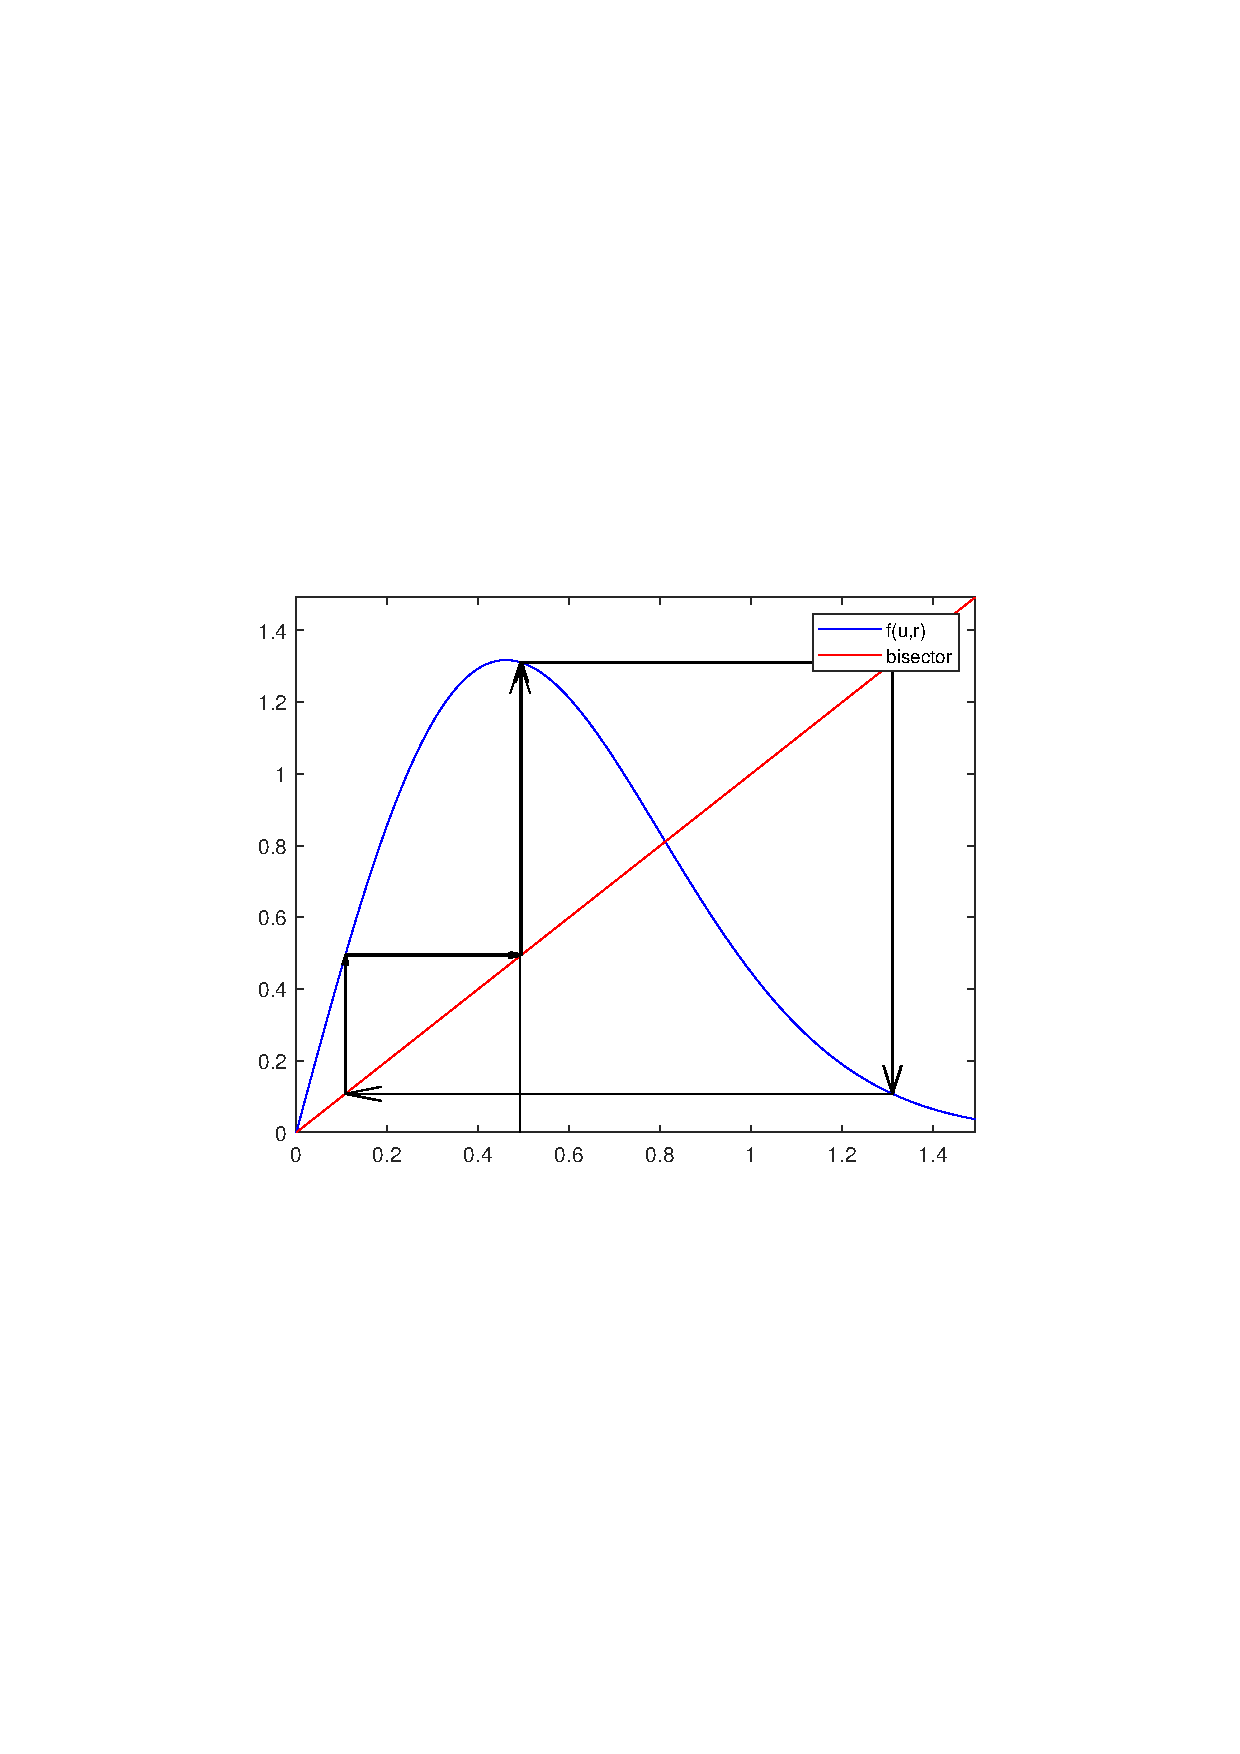
\includegraphics[width=7cm]{cicle3.pdf} }}
    \caption{Цикл длины три. \( r = 4.717, u_1 = 0.107, u_2 = 0.492, u_3 = 1.310 \) }
\end{figure}
 
По теореме Шарковского наличие при некоторых значених параметров в системе цикла длины три влечет за собой наличие циклов всех длин, и значит цикла длины два. Для наглядности найдем и изобразим устойчивый цикл длины два, поэтому рассмотрим всё же другое значение параметра \( r \), нежели то, что было использовано для демонстрации цикла длины три.

Установить значения параметра и точки цикла длины два легко, рассмотрев внимательнее бифуркационную диаграмму и построив график \( f^2 = f \circ f \). \\
Решим уравнение \(f^2(u) = u \). Фиксируем, например, параметр \( r = 3.2 \)(на бифуркационной диаграмме видно, что в этом случае имеется устойчивый цикл длины два) и найдем точки цикла:
\[ u_1 = 0.532, u_2 = 1.082. \]

\begin{figure}[h]
    \centering
    \subfloat[\centering График \( f^2 \) с тремя точками пересечения биссектрисы первого координатного угла, крайние из которых являются точками цикла, а средняя неподвижной точкой для функции \( f^1 \).]{{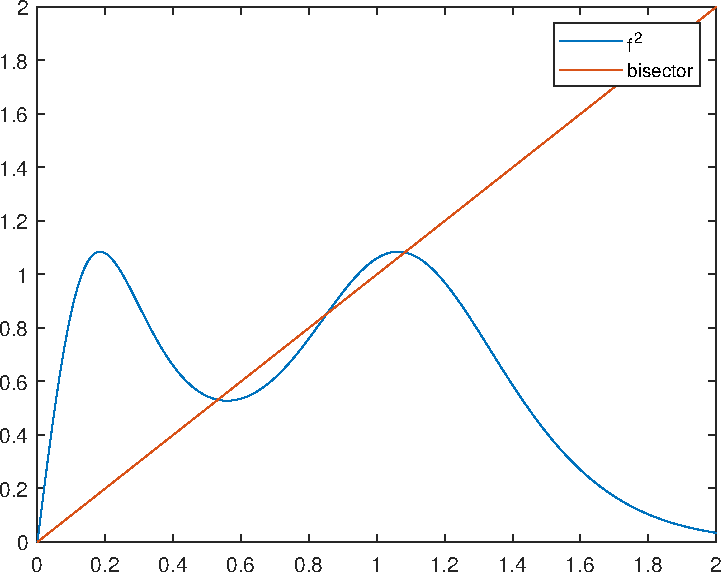
\includegraphics[width=7cm]{f2.pdf} }}
    \qquad
    \subfloat[\centering Траектория системы, соответствующая устойчивому чиклу длины два.]{{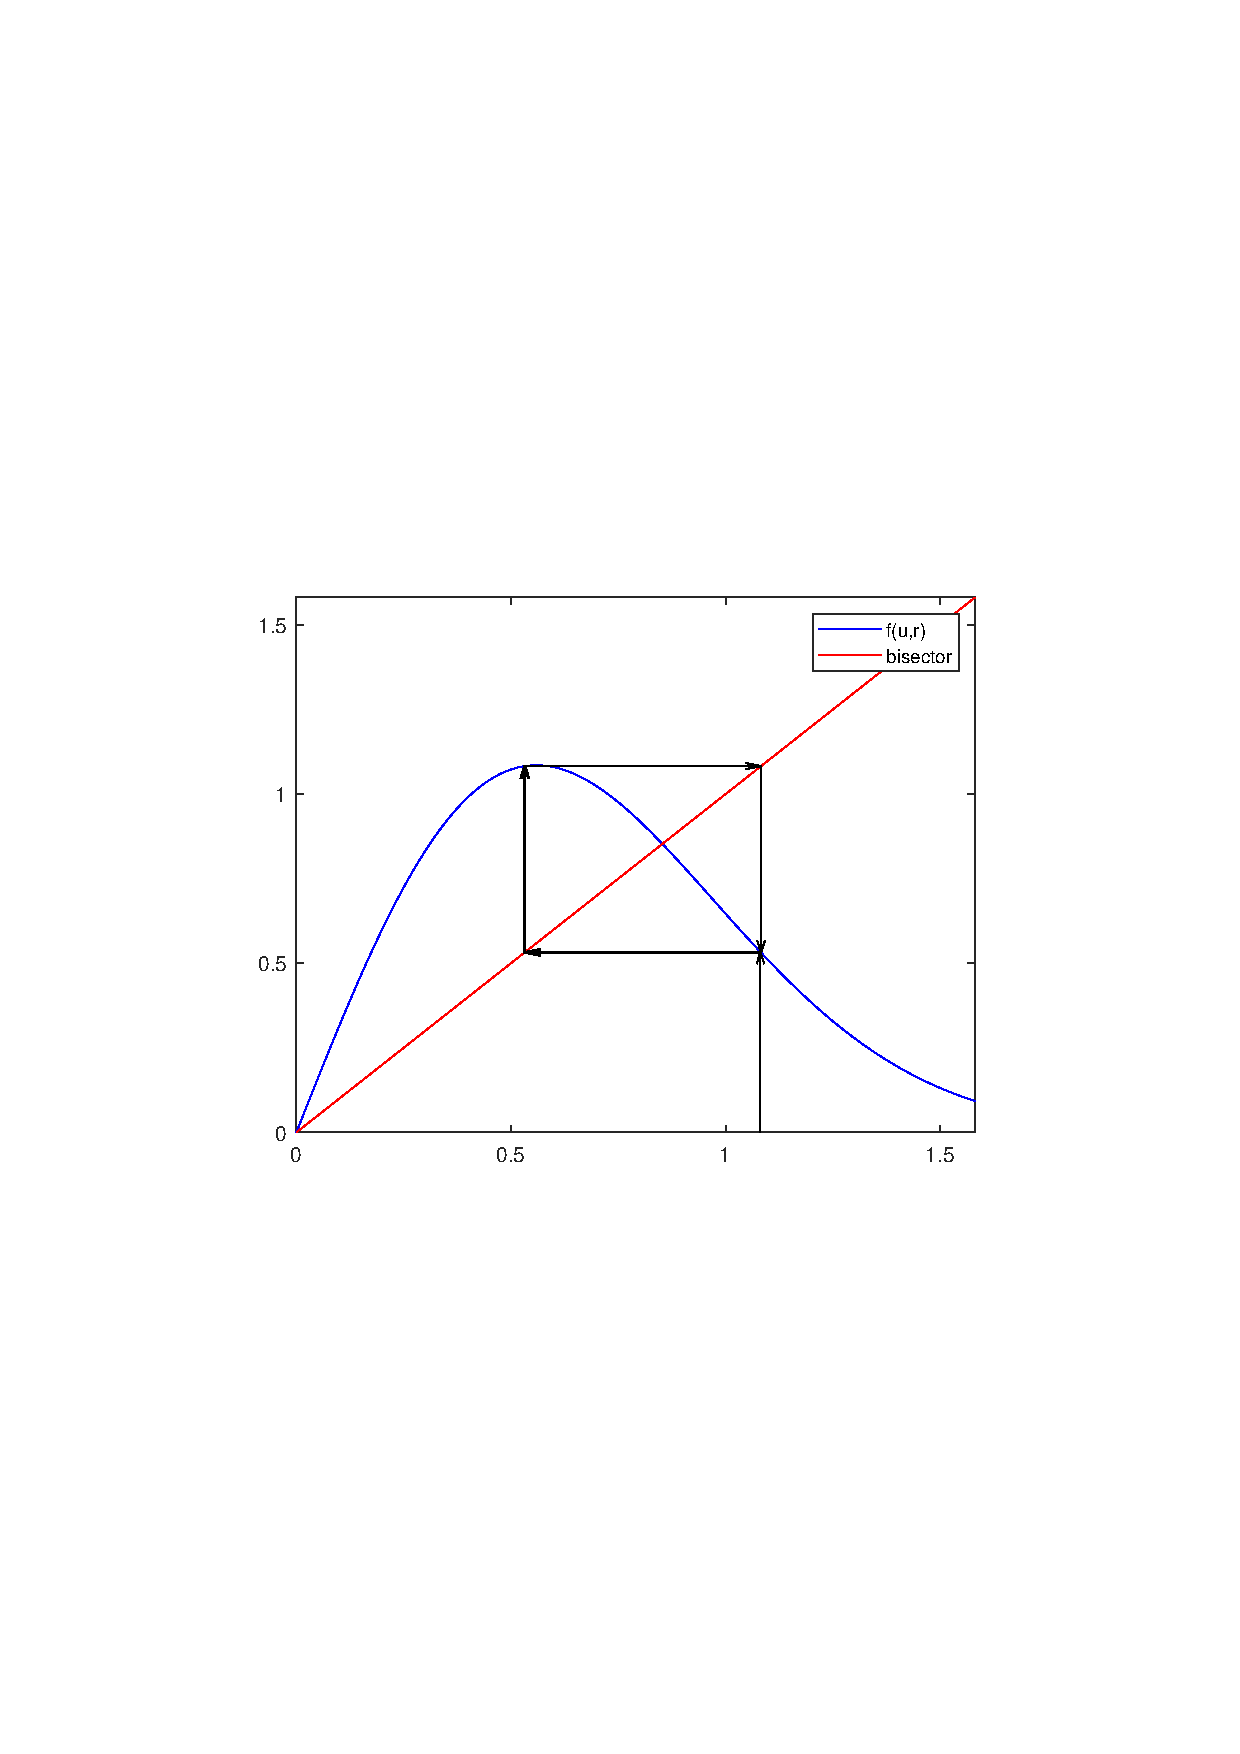
\includegraphics[width=7cm]{cicle2.pdf} }}
    \caption{Цикл длины два. \(  r = 3.2, u_1 = 0.532, u_2 = 1.082 \) }
\end{figure}
	
\anonsubsubsection{Зависимость показателя Ляпунова от параметров системы}
Как и ранее, введем для начала необходимые определения:
\begin{definition}
	Пусть \( f : \mathbb{R} \to \mathbb{R} \) --- гладкое отображение. Числом Ляпунова траектории \( u_1, u_2, \dots, u_n, \dots \)  называется величина
	\[ l(u_1) = \lim\limits_{n \to \infty} (|f'(u_1)| \cdot |f'(u_2)| \cdot \dots \cdot |f'(u_n)|)^{\frac{1}{n}}, \]
	если этот предел существует.
\end{definition}


\begin{definition}
	Пусть \( f : \mathbb{R} \to \mathbb{R} \) --- гладкое отображение. Показателем Ляпунова траектории \( u_1, u_2, \dots, u_n, \dots \) называется величина
	\[ h(u_1) = \lim\limits_{n \to \infty} \frac{\ln|f'(u_1)| + \ln|f'(u_2)| + \dots + \ln|f'(u_n)|}{n}, \]
	если этот предел существует.
\end{definition}

Число и показатель Ляпунова характеризуют поведение ``близких'' траекторий при изменении дискретной величины \( t \). Действительно, пусть \( u_1 \) и \( \overline{u}_1 \) --- две достаточно близкие начальные точки гладкого отображения \( f \). Эти точки порождают две орбиты динамической системы, заданной отображением \( f \):
\[ u_1, u_2, \dots, u_k, \dots \ ; \ \overline{u}_1, \overline{u}_2, \dots, \overline{u}_k, \dots .\]
Для точек второй итерации \( u_2 \) и \( \overline{u}_2 \) выполнено:
\[ u_2 - \overline{u}_2 = f(u_1) - f(\overline{u}_1) = f'(u_1)(u_1 - \overline{u}_1) + o(|u_1 - \overline{u}_1|) .\]
Если \( |f'(u_1)| < 1 \), то в линейном приближении расстояние между точками \( u_2 \) и \( \overline{u}_2 \) будет меньше, чем расстояние между начальными точками \( u_1\) и \( \overline{u}_1 \). В противном случае расстояние по сравнению с начальным положением увеличится. Аналогичные рассуждения справедливы для всех итераций \( t \). Число и показатель Ляпунова представляют из себя некоторое среднее значение производной на каждой из итераций, поэтому считаются мерой близости орбит. Если число Ляпунова больше единицы(показатель Ляпунова больше нуля), то близкие орбиты в среднем расходятся, иначе --- сходятся. 

Построим график зависимости показателя Ляпунова от значения параметра \( r \). Для этого для каждого значения параметра \( r \) из некоторой сетки проведем n итераций системы, и на каждой итерации будем вычислять значение производной функции \( f \) в полученной точке. Сложим прологарифмированные модули вычисленных значений производных и поделим на n. При достаточно больших n полученное значение можно приближенно считать пределом по n, стоящим в определении показателя Ляпунова.

\begin{figure}[h]
	\center{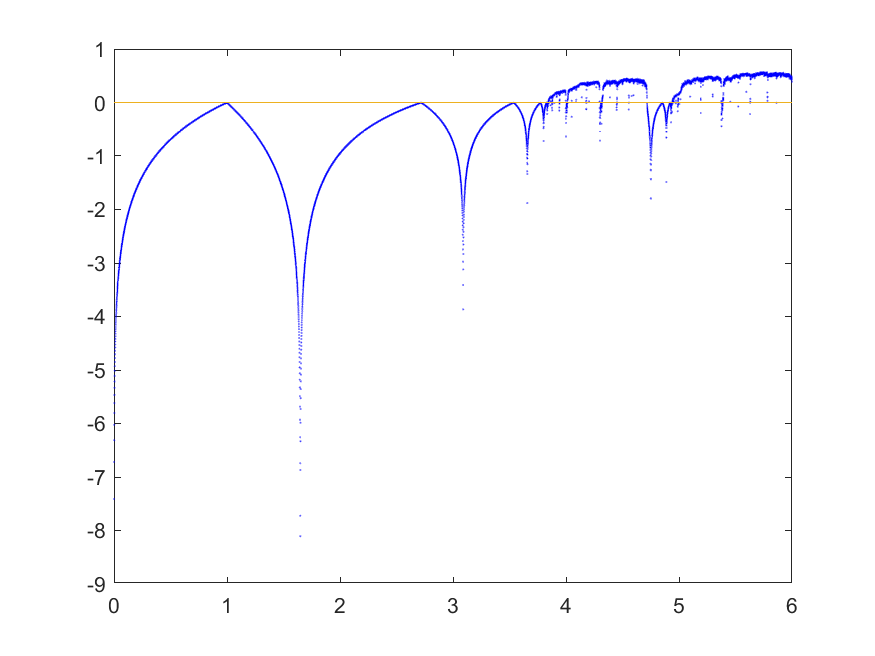
\includegraphics[scale = 0.8]{lyapunov_exponent.pdf}}
	\caption{Зависимость показателя Ляпунова от значения параметра \( r \). (\ref{first_system}). n = 1000}
\end{figure}

Полезно сравнить бифуркационную диаграмму и график показателя Ляпунова. В точках, где показатель Ляпунова имеет отрицательные значения, на бифуркационной диаграмме четко видны устойчивые неподвижные точки или устойчивые предельные циклы. Где показатель Ляпунова больше нуля наблюдается хаотическое поведение траекторий.

\anonsubsection{Исследование двухшаговой системы}
Теперь рассмотрим систему с запаздыванием (\ref{second_system}):
\[ u_{t+1} = ru_te^{-\frac{r}{2}u_{t-1}^2} \ , \ u_t> 0 \ , \ \forall t \in \mathbb{N} \]

\noindent Система с запаздыванием сводится к многомерной дискретной системе вида:
\begin{equation}\label{multidimensional_system}
	\begin{cases}
		u_{t+1} = f_1(u_t, v_t) = ru_te^{-\frac{r}{2}v_t^2} \\
		v_{t+1} = f_2(u_t, v_t) = u_t.
	\end{cases}
\end{equation}
В дальнейшем мы будем работать именно с ней.
\anonsubsubsection{Нахождение неподвижных точек}
В случае многомерных систем неподвижная точка определяется следующим образом:
\begin{definition}
	Точка \( u^* \in \mathbb{R}^n\) называется неподвижной точкой многомерной дискретной системы \( u_{t+1} = f(u_t) \ , \ u_t \in \mathbb{R}^n \ , \ f:\mathbb{R}^n \to \mathbb{R}^n\), если \(u^* = f(u^*).\)
\end{definition}

В случае системы с запаздыванием, которую мы предварительно свели к многомерной, это означает что точка \( u^* \) может считаться устойчивой, если \( u^* = f(u^*, u^*, \dots, u^*) \), где \( u^* \in \mathbb{R} \ , \ f: \mathbb{R}^n \to \mathbb{R} \). Тогда неподвижные точки для соответствующей многомерной системы будут иметь вид \( u = \underbrace{(u^*, u^*, \dots, u^*)}_n. \)

Таким образом для нахождения неподвижных точек можно аналогично первому пункту решить относительно \( u \) уравнение:
\[ f_1(u, u) = u \ , \ u \in \mathbb{R} \ , \ r > 0 , \]
или с учетом конкретной системы
\[ rue^{-\frac{r}{2}u^2} = u \ , \ u \in \mathbb{R} \ , \ r > 0 . \]
В итоге получим две неподвижные точки многомерной системы  (\ref{multidimensional_system})
\[ u_1^* = (0, 0)^\mathrm{T} \ , \ u_2^* = \bigg(\sqrt{\frac{2\ln r}{r}}, \sqrt{\frac{2\ln r}{r}}\bigg)^\mathrm{T} .\]

\anonsubsubsection{Исследование характера неподвижных точек}
Для исследования неподвижных точек многомерной системы требуется следующая теорема:
\begin{theorem}
	Пусть задана многомерная динамическая система с дискретным временем:
	\[ u_{t+1}  = f(u_t) \ , \ u_t \in \mathbb{R}^n \ , \ t \in \mathbb{N} , \]
	где \( f \) --- гладкое отображение из \( \mathbb{R}^n \) в \( \mathbb{R}^n \), и \( u^* \) --- неподвижная точка данной системы. Тогда \( u^* \) ассимптотически устойчива, если все собственные значения \( \lambda_1, \lambda_2, \dots, \lambda_n \) матрицы Якоби функции \( f(u) \) в точке \( u^* \) удовлетворяет условию \( |\lambda_i| < 1, i = 1, 2, \dots, n \). Если модуль хотя бы одного собственного значения больше единицы, то \( u^* \) неустойчива.
\end{theorem}

Выпишем матрицу Якоби для системы (\ref{multidimensional_system}):
\begin{equation}
	\mathcal{J}(u,v) = \begin{pmatrix} \frac{\partial f_1}{\partial u} & \frac{\partial f_1}{\partial v} \smallskip\\  \frac{\partial f_2}{\partial u} & \frac{\partial f_2}{\partial v}\end{pmatrix} = \begin{pmatrix} re^{-\frac{r}{2} v^2(t)} & -r^2u(t)v(t)e^{-\frac{r}{2}v^2(t)} \smallskip\\ 1 & 0 \end{pmatrix}.
\end{equation}

\begin{enumerate}
	\item При \( u_1^* = (0,0)^\mathrm{T} \):
	\[\mathcal{J}(u_1^*) = \begin{pmatrix} r & 0 \smallskip\\ 1 & 0 \end{pmatrix} \] \\
	\[ \mathrm{det} ( \mathcal{J}(u_1^*) - \lambda \mathrm{E}) = \begin{vmatrix} r - \lambda & 0 \\ 1 & -\lambda \end{vmatrix} = \lambda(\lambda - r)  \implies \lambda_1 = 0, \lambda_2 = r\]
	Таким образом по теореме 2 точка \( u_1^* = (0, 0)^{\mathrm{T}} \) устойчива при \( r < 0 \). В остальных случаях точка является неустойчивой.
	\item При \( u_2^* = \bigg(\sqrt{\frac{2\ln r}{r}}, \sqrt{\frac{2\ln r}{r}}\bigg)^\mathrm{T} \):
	\[ \mathcal{J}(u_2^*) = \begin{pmatrix} re^{-\ln r} & -2r\ln r e^{-\ln r} \\ 1 & 0 \end{pmatrix}  = \begin{pmatrix} 1 & -2\ln r \\ 1 & 0 \end{pmatrix}. \]\\
	\[ \mathrm{det} (\mathcal{J} (u_2^*) - \lambda \mathrm{E} ) = \begin{vmatrix} 1 - \lambda & -2\ln r \\ 1 & -\lambda \end{vmatrix} = \lambda (\lambda - 1) + 2 \ln r = \lambda^2 - \lambda + 2 \ln r. \]
	\[ D = 1 - 8 \ln r \implies \lambda_{1,2} = \frac{1 \pm \sqrt{1 - 8 \ln r}}{2}\]
	\begin{enumerate}
		\item При \( 1 - 8 \ln r \ge 0 \iff r \le e^\frac{1}{8}\) собственные значения матрицы Якоби действительны.
		Так как \( \lambda_1 = \frac{1 + \sqrt{1 - 8 \ln r}}{2} > \frac{1 - \sqrt{1 - 8 \ln r}}{2} = \lambda_2 \) возможно получить границы в которых оба собственных значения по модулю меньше единицы из неравенств:
		\[ \begin{cases} \lambda_1 = \frac{1 + \sqrt{1 - 8 \ln r}}{2} < 1 \\ \lambda_2 = \frac{1 - \sqrt{1 - 8 \ln r}}{2} > -1 \end{cases} \iff \begin{cases} r > 1 \\ r > \frac{1}{e} \end{cases}. \]
		Тогда \( |\lambda_{1,2} | < 1 \) при \( r > 1 \). То есть для вещественных собственных значений точка \( u_2^* \) устойчива при \( r \in (1;e^\frac{1}{8}] \).
		\item При \( 1 - 8 \ln r < 0 \iff r > e^\frac{1}{8} \) собственные значения комплексные и имеют вид \( \lambda_{1,2} = \frac{1 \pm i\sqrt{8 \ln r - 1}}{2} \).
		\[ | \lambda_{1,2} | = \sqrt{\frac{1}{4} + \frac{8 \ln r - 1}{4} } = \sqrt{2 \ln r } \le 1 \iff r \le \sqrt{e} \]
	То есть для комплексных собственных значений точка \( u_2^* \) устойчива при \( r \in (e^\frac{1}{8}; e^\frac{1}{2}) \). 
	\end{enumerate}
	В итоге получим, что точка \( u_2^* \) устойчива при \( r \in (1;e^\frac{1}{2} ) \). В остальных случаях точка является неустойчивой.
\end{enumerate}

\anonsubsubsection{Нахождение бифуркации Неймарка-Сакера}
	Бифуркация Неймарка-Сакера это дискретный аналог бифуркации Андронова-Хопфа рождения инвариантной кривой. При переходе через критическое значение параметра, в окрестности неподвижной точки появляется инвариантная кривая(транскритическая бифуркация), либо инвариантная кривая существует ``до'' бифуркации(субкритическая бифуркация). Стоит отметить, что для появления такой бифуркации существенны условия невырожденности, которые приведены в \cite{1} \footnote{Приложение А.8, стр. 421}. При нарушении одного из этих условий возможно как отсутствие инвариантной кривой, так и появление нескольких кривых. \medskip\\
	Рассмотрим двумерную динамическую систему с дискретным временем
	\begin{equation}\label{two-dimensional system}
		u \mapsto f(u,r) \ , \ u = (u_1, u_2) \in \mathbb{R}^2 \ , \ r \in \mathbb{R} \ , \ f : \mathbb{R}^3 \to \mathbb{R}^2 . 
	\end{equation}
	
\begin{definition}
	Бифуркация положения равновесия в системе (\ref{two-dimensional system}), соответствующая появлению мультипликаторов \( |\lambda_1| = |\lambda_2| = 1, \lambda_1 = \overline{\lambda}_2 \), называется бифуркацией Неймарка-Сакера или дисретной бифуркацией Хопфа.
\end{definition}
В данном определении под мультипликаторами понимаются собственные значения матрицы Якоби дискретной многомерной системы.\medskip\\
В случае данной системы такие собственные значения появляются у матрицы Якоби для точки \( u_2^* \) при значении параметра \( r = e^\frac{1}{2} \).
При этом из предыдущего пункта видно, что неподвижная точка при переходе через критическое значение из устойчивой превращается в неустойчивую. 
В окрестности точки \( u_2^* \) появляется устойчивый цикл, то есть устойчивая неподвижная точка сменяется устойчивым предельным циклом малой длины, поэтому система остается в окрестности этой точки. Это так называемая магкая или некатострофическая потеря устойчивости.

\begin{figure}[h]
    \centering
    \subfloat[\centering Сходимость траектории к неподвижной точке при значении параметра меньшем критического. \( r = 1.6287 \)]{{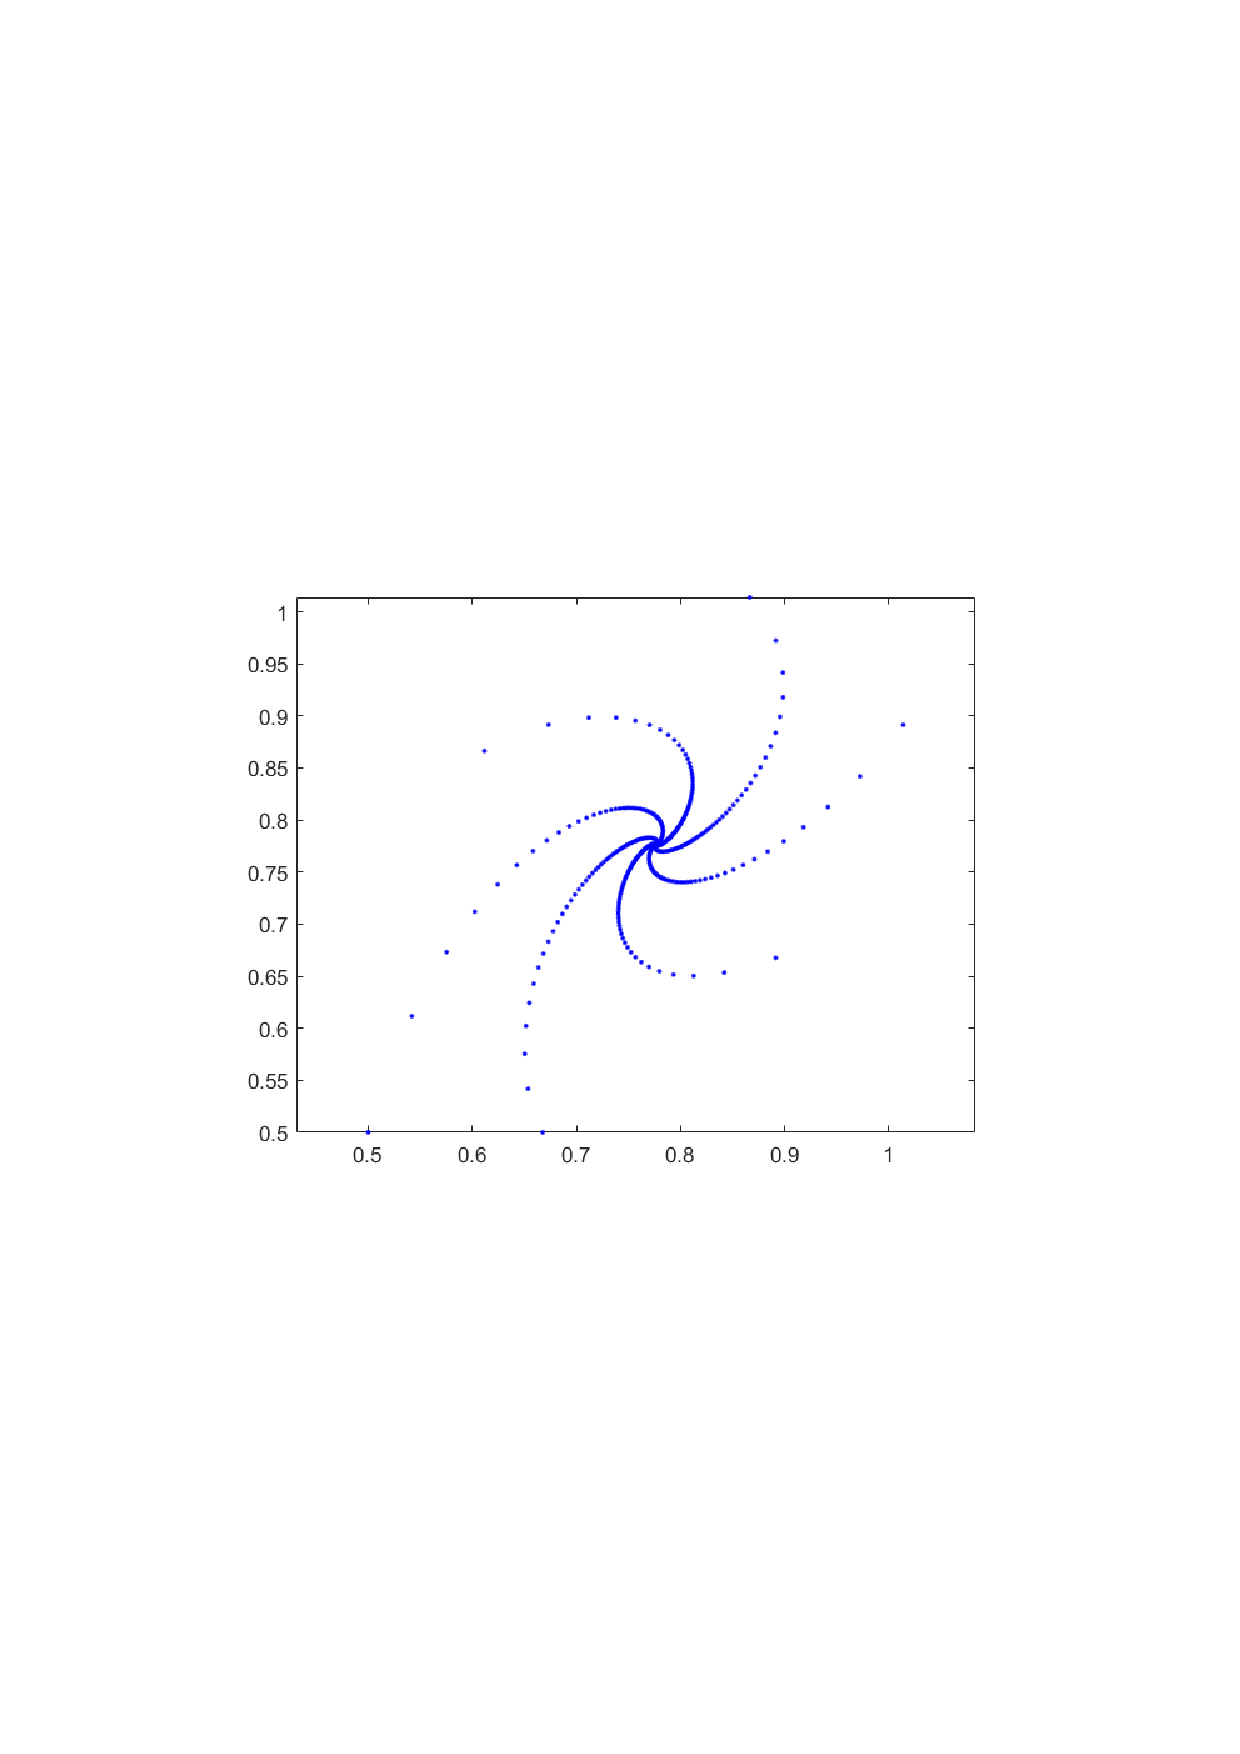
\includegraphics[width=7cm]{before_bifurcation.pdf} }}
    \qquad
    \subfloat[\centering Появление устойчивого предельного цикла после прохождения параметром критического значения. \( r = 1.6587 \)]{{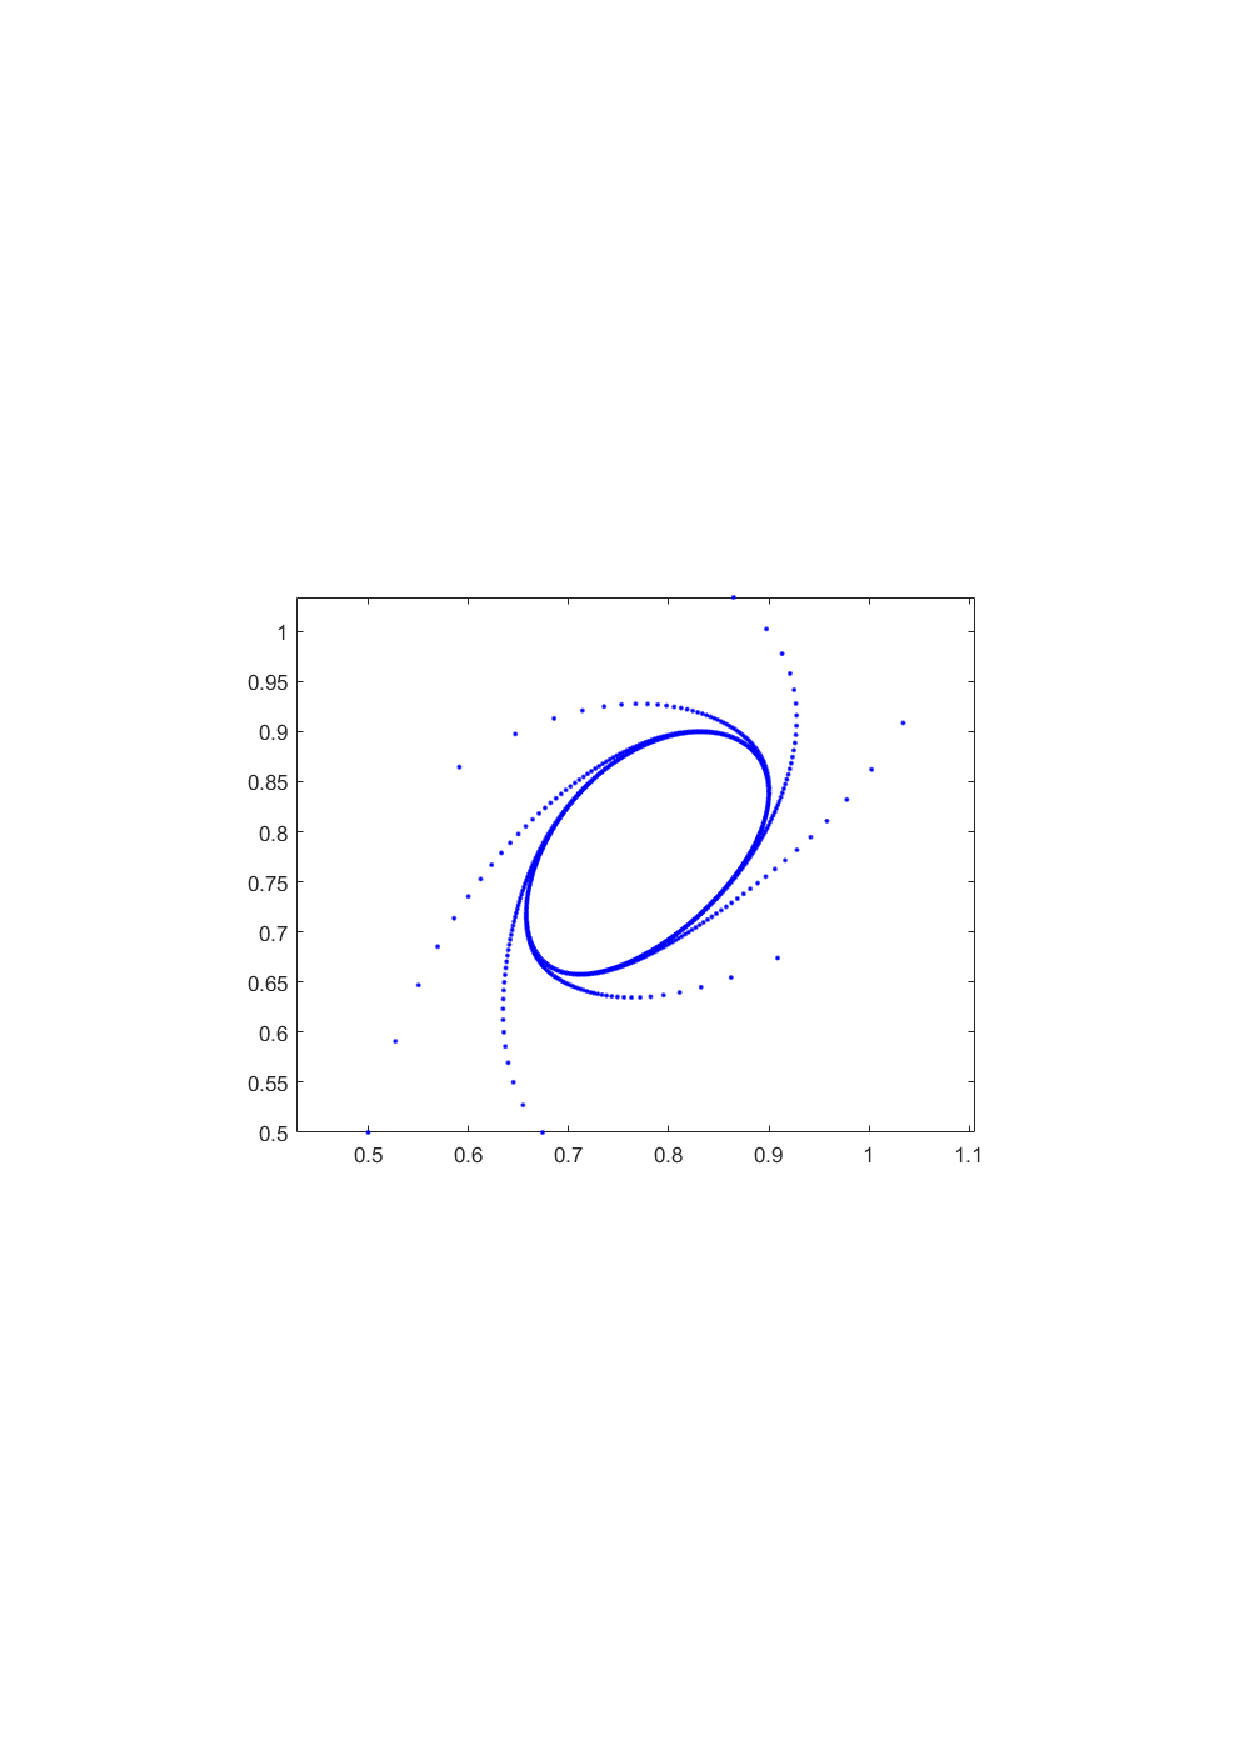
\includegraphics[width=7cm]{after_bifurcation.pdf} }}
    \caption{Иллюстрация появления в окрестнсости точки \( u_2^* \) устойчивого цикла.}
\end{figure}
\newpage
\anonsection{Динамические системы с непрерывным временем}
\anonsubsection{Постановка задачи}
\setcounter{section}{2}
\setcounter{equation}{0}
\setcounter{definition}{0}
\setcounter{theorem}{0}

Дана динамическая система на плоскости с непрерывным временем:
\begin{equation}
	\begin{cases} \dot{x} = \frac{ax(K - x)}{K} - bxy, \\ \dot{y} = -cy + \frac{dxy^2}{1+Ay}, \end{cases} (x,y) \in \mathbb{R}_2^+;
\end{equation}
Все параметры считаются положительными. \medskip\\

Необходимо:
\begin{enumerate}
	\item Дать биологическую интерпретацию характеристик системы.
	\item Ввести новые безразмерные переменные, уменьшив число входящих в систему параметров.
	\item Найти неподвижные точки системы и исследовать их характер в зависимости от значений параметров. Результаты исследования представить в виде параметрического портрета системы.
	\item Для каждой характерной области параметрического портрета построить фазовый портрет. Дать характеристику поведения системы в каждом из этих случаев.
	\item Исследовать возможность возникновения предельного цикла. В положительном случае найти соответствующее первое ляпуновское число. Исследовать характер предельного цикла.
	\item Дать биологическую интерпретацию полученным результатам.
\end{enumerate}
\anonsubsection{Биологическая интерпретация системы}
Данная система описывает взаимодействие двух популяций, ``хищников'' и ``жертв''. Под \( x \) можно понимать численность популяции жертв, а под \( y \) --- численность хищников. 
\begin{itemize}
	\item Первое слагаемое \( \frac{ax(K - x)}{K} \) представляет собой скорость роста популяции жертв в отсутствие хищников с учетом внутривидовой конкуренции. Здесь \( K \) --- максимальное количество жертв, \( a \) --- коэффициент, имеющий смысл скорости роста жертв, однако при приближении численности к \( K \) рост постепенно замедляется. 
	\item Второе слагаемое \( -bxy \) --- это уменьшение скорости прироста жертв в зависимости от их числа и числа хищников. Иными словами, сколько хищники могут съесть жертв при определенном числе жертв и хищников. 
	\item Слагаемое \( -cy \) отвечает за скорость вымирания хищников в отстутсвие жертв. 
	\item Последнее слагаемое \( \frac{dxy^2}{1 + Ay} \) несет смысл скорости прироста популяции хищников в зависимости от их числа и числа жертв. В некотором смысле представляет собой функцию ``полезности'' поедания жертв хищниками.
\end{itemize}

\anonsubsection{Введение новых безразмерных переменных}
Чтобы уменьшить число параметров, входящих в систему сделаем замену переменных:
\[ x(t) = pu(\tau) \ , \ y(t) = qv(\tau) \ , \ t = \frac{\tau}{T}, \]
где \( p \) и \( q \) пока неизвестные константы. Тогда получим:
\[ \dot{x} = p \cdot \frac{du(\tau)}{d\tau} \cdot \frac{d\tau}{dt} = p \cdot \dot{u}(\tau) \cdot T \ , \ \dot{y} = q \cdot \frac{dv(\tau)}{d\tau} \cdot \frac{d\tau}{dt} = p \cdot \dot{v}(\tau) \cdot T\]
Здесь и далее под \( \dot{u} \) и \( \dot{v}\) понимается производная \( u \) и \( v \) по \( \tau \). Подставим теперь новые переменные в систему.
\[ \begin{cases} p\dot{u}T = \frac{apu(K - pu)}{K} - bpquv, \medskip\\ q\dot{v}T = -cqv + \frac{dpuq^2v^2}{1 + Aqv}, \end{cases} \iff \begin{cases} \dot{u}T = \frac{au(K - pu)}{K} - bquv, \medskip\\ \dot{v}T = -cv + \frac{dpquv^2}{1+Aqv}, \end{cases} \iff \begin{cases} \dot{u}T = u \Big( \frac{a(K - pu)}{K} - bqv \Big), \medskip\\ \dot{v}T = -cv + \frac{dpquv^2}{1+Aqv}. \end{cases} \]
Пусть \( T = a , q = \frac{a}{b} \). Тогда для первого уравнения получим:
\[ \dot{u}a = u\Big(\frac{a(K - pu)}{K} - av\Big) \iff \dot{u} = u(1 - \frac{p}{K}u - v). \]
Преобразуем второе уравнение:
\[ \dot{v}T = -cv + \frac{dpquv^2}{1+Aqv} \iff \dot{v}a = -cv + \frac{dp \cdot \frac{a}{b} uv^2}{1+A \cdot \frac{a}{b} v} \iff \dot{v} = -\frac{c}{a}v + \frac{\frac{dp}{aA}uv^2}{\frac{b}{Aa} + v} . \] 
Потребуем, чтобы \( \frac{dp}{aA} = 1 \), таким образом получим \( p = \frac{aA}{d} \), тогда:
\[ \dot{v} = -\frac{c}{a}v + \frac{uv^2}{\frac{b}{Aa} + v} .\]
В итоге имеем:
\[ q = \frac{a}{b} \ , \ p = \frac{aA}{d} \ , \ t = \frac{\tau}{a}. \]
То есть приходим к замене:
\[ x(t) = \frac{aA}{d}u(\tau) \ , \ y(t) = \frac{a}{b}v(\tau) \ , \ t = \frac{\tau}{a}, \]
после которой система приобретает вид:
\[  \begin{cases} \dot{u} = u( 1 - \frac{aA}{dK}u - v), \medskip\\ \dot{v} = -\frac{c}{a}v + \frac{uv^2}{\frac{b}{Aa} + v}. \end{cases} \]
Обозначив \( \frac{aA}{dK} = \alpha \ , \ \frac{c}{a} = \beta \ , \ \frac{b}{Aa} = \gamma \), окончательно, имеем систему:
\begin{equation}\label{new_system}
	\begin{cases}
		\dot{u}(\tau) = u(\tau)(1 - \alpha u(\tau) - v(\tau)), \\
		\dot{v}(\tau) = -\beta v(\tau) + \frac{u(\tau)v^2(\tau)}{\gamma + v(\tau)}.
	\end{cases}
\end{equation}
Таким образом мы свели исходную систему с шестью параметрами к системе с тремя параметрами. Теперь можем приступить к анализу неподвижных точек.
\anonsubsection{Неподвижные точки преобразованной системы}
Рассмотрим систему
\begin{equation}\label{rn_system}
	\dot{x} = f(x) \ , \ x \in \mathbb{X} \subseteq \mathbb{R}^n \ , \ f : \mathbb{X} \to \mathbb{R}^n.
\end{equation}

\begin{definition}
	Неподвижной точкой системы (\ref{rn_system}) называется точка \( x^* \in \mathbb{X} \), такая что \( f(x^*) = 0 \).
\end{definition}

\noindent Таким образом, для поиска неподвижных точек рассмотрим систему:
\[ \begin{cases} 
	u(1 - \alpha u - v) = 0, \\ 
	-\beta v + \frac{uv^2}{\gamma + v} = 0 .
\end{cases} \]
Для первого уравения:
\[ u(1 - \alpha u - v) = 0 \iff \left[ \begin{array}{l} u = 0, \\ 1 - \alpha u - v = 0. \\ \end{array} \right. \]
\begin{enumerate}
	\item В первом случае имеем:
	\[ \begin{cases} u = 0 , \\ -\beta v + \frac{uv^2}{\gamma + v} = 0, \end{cases}  \iff \begin{cases} u =  0 , \\ -\beta v = 0, \end{cases} \iff \begin{cases} u = 0, \\ v = 0. \end{cases} \]
	То есть получаем первую неподвижную точку \( u_1^* = (0, 0)^{\mathrm{T}} \), которая существует при любых значениях параметров.
	\item Во втором случае имеем:
	\[\begin{cases} u = \frac{1 - v}{\alpha}, \\ -\beta v + \frac{uv^2}{\gamma + v} = 0. \end{cases}  \]
	Найдем отсюда \( v \). 
	\[ -\beta v + \frac{\frac{1 - v}{\alpha}v^2}{\gamma + v} = v\Big(-\beta + \frac{\frac{1 - v}{\alpha} v}{\gamma + v}\Big) = 0 \iff \left[ \begin{array}{l} v = 0, \smallskip\\ \frac{\frac{1 - v}{\alpha} v}{\gamma + v} = \beta. \\ \end{array} \right.\]
	Таким образом получим две системы:
	\[ \begin{cases} u = \frac{1 - v}{\alpha} , \\ v = 0, \end{cases} \text{и}  \quad \begin{cases} u = \frac{1 - v}{\alpha}, \\ \frac{\frac{1 - v}{\alpha} v}{\gamma + v} = \beta. \end{cases} \]
	Из первой немедленно получаем вторую неподвижную точку \( u_2^* = (\frac{1}{\alpha}, 0)^{\mathrm{T}} \), которая также существует при любых положительных значениях параметров. Вторую систему рассмотрим подробнее. Преобразуем второе уравнение:
	\[ -\beta + \frac{\frac{1 - v}{\alpha} v}{\gamma + v} = -\beta + \frac{v - v^2}{\alpha \gamma + \alpha v} = \frac{-\alpha \beta \gamma - \alpha \beta v + v - v^2}{\alpha (\gamma + v)} \]
	Тогда 
	\[ \frac{-\alpha \beta \gamma - \alpha \beta v + v - v^2}{\alpha (\gamma + v)} = 0 \iff \frac{v^2 + v(\alpha \beta - 1) + \alpha \beta \gamma}{\alpha (\gamma + v)} = 0 \iff \]
	\[\iff \begin{cases} v^2 + v(\alpha \beta - 1) + \alpha \beta \gamma = 0, \\ \alpha (\gamma + v) \ne 0 \end{cases} \]
	Второе неравенство выполнено при любых положительных значениях параметров. Первое равенство в системе представляет из себя квадратное уравнение относительно \( v \). Найдем его корни:
	\[ \mathrm{D} = (\alpha \beta - 1)^2 - 4 \alpha \beta \gamma = \implies v = \frac{1 - \alpha \beta \pm \sqrt{(\alpha \beta - 1)^2 - 4 \alpha \beta \gamma}}{2} \]
	Таким образом получим еще две неподвижные точки, которые существуют при \( \mathrm{D} > 0 \) и сливаются в одну при \( \mathrm{D} = 0 \).
	\[ u_3^* =  \Big( \frac{1 + \alpha \beta + \sqrt{(\alpha \beta - 1)^2 - 4 \alpha \beta \gamma}}{2\alpha},  \frac{1 - \alpha \beta - \sqrt{(\alpha \beta - 1)^2 - 4 \alpha \beta \gamma}}{2} \Big)^{\mathrm{T}}, \] 
	\[ u_4^* =  \Big( \frac{1 + \alpha \beta - \sqrt{(\alpha \beta - 1)^2 - 4 \alpha \beta \gamma}}{2\alpha},  \frac{1 - \alpha \beta + \sqrt{(\alpha \beta - 1)^2 - 4 \alpha \beta \gamma}}{2} \Big)^{\mathrm{T}}. \]
	Найдем, условия, при которых \( \mathrm{D} \geq 0 \).
	\[ \mathrm{D} = (\alpha \beta - 1)^2 - 4 \alpha \beta \gamma \ge 0 \iff (\alpha \beta)^2 - 2 \alpha \beta + 1 - 4 \alpha \beta \gamma \ge 0 \iff \alpha \beta ( \alpha \beta - 2 - 4 \gamma) \ge -1. \]
Однако при этом из вида \( u = \frac{1 - v}{\alpha} \) и условия неотрицательности \( u \) и \( v \) получим, что ,чтобы эти точки принадлежали фазовому пространству \( \mathbb{U} = \{(u,v) \in \mathbb{R}^2 : u \ge 0, v \ge 0 \} \), требуется \( 0 \le v \le 1 \). Получим условия, при которых это выполнено(учитывая выполнение условия неотрицательности дискриминанта).\\
Для \( u_3^* \):
\begin{itemize}
	\item Условие \( v \geq 0 \):
	\[ \frac{1 - \alpha \beta - \sqrt{(\alpha \beta - 1)^2 - 4\alpha \beta \gamma}}{2} \geq 0 \iff \begin{cases} (1 - \alpha \beta)^2 \geq (\alpha \beta - 1)^2 - 4 \alpha \beta \gamma, \\ \alpha \beta < 1, \end{cases} \iff \] 
	\[ \iff \begin{cases} 4 \alpha \beta \gamma \geq 0, \\ \alpha \beta < 1, \end{cases} \iff \alpha \beta < 1. \]	
	\item Условие \( v \leq 1 \):
	\[ \frac{1 - \alpha \beta - \sqrt{(\alpha \beta - 1)^2 - 4\alpha \beta \gamma}}{2} \leq 1 \iff -1 - \alpha \beta \leq \sqrt{(\alpha \beta - 1)^2 - 4 \alpha \beta \gamma}. \]
\end{itemize}
Отметим, что второе условие выполняется для любых положительных значений параметров.\\
Для \( u_4^* \):
\begin{itemize}
	\item Условие \( v \geq 0 \):
	\[ \frac{1 - \alpha \beta - \sqrt{(\alpha \beta - 1)^2 - 4\alpha \beta \gamma}}{2} \geq 0 \iff \alpha \beta - 1 \leq \sqrt{(\alpha \beta - 1)^2 - 4 \alpha \beta \gamma}, \]
	что очевидно выполнено при \( \alpha \beta < 1 \). Для \( \alpha \beta \geq 1 \) получим:
	\[ \alpha \beta - 1 \leq \sqrt{(\alpha \beta - 1)^2 - 4 \alpha \beta \gamma} \iff 4 \alpha \beta \gamma \leq 0, \]
	Что невозможно при положительных значениях параметров. Таким образом получим так же что \( v \geq 0 \iff \alpha \beta < 1 \). 
	\item Условие \( v \leq 1 \):
	\[ \frac{1 - \alpha \beta + \sqrt{(\alpha \beta - 1)^2 + 4\alpha \beta \gamma}}{2} \leq 1 \iff \alpha \beta + 1 \geq \sqrt{(\alpha \beta - 1)^2 - 4 \alpha \beta \gamma} \iff 4 \alpha \beta > -4 \alpha \beta \gamma, \]
	что также выполнено при любых положительных значениях параметров.
\end{itemize}
\end{enumerate} 
Таким образом, у системы существует четыре положения равновесия:
\[ u_1^* = (0, 0)^{\mathrm{T}} \ , \ u_2^* = (\frac{1}{\alpha}, 0)^{\mathrm{T}} \]
\[ u_3^* =  \Big( \frac{1 + \alpha \beta + \sqrt{(\alpha \beta - 1)^2 - 4 \alpha \beta \gamma}}{2\alpha},  \frac{1 - \alpha \beta - \sqrt{(\alpha \beta - 1)^2 - 4 \alpha \beta \gamma}}{2} \Big)^{\mathrm{T}}, \]
\[ u_4^* =  \Big( \frac{1 + \alpha \beta - \sqrt{(\alpha \beta - 1)^2 - 4 \alpha \beta \gamma}}{2\alpha},  \frac{1 - \alpha \beta + \sqrt{(\alpha \beta - 1)^2 - 4 \alpha \beta \gamma}}{2} \Big)^{\mathrm{T}}. \]
Первые два из которых существуют при любых значениях параметров, третье и четвертое появляются при условии \( \alpha \beta ( \alpha \beta - 2 - 4 \gamma) \ge -1 \), вместе с условием \( \alpha \beta < 1 \).
\anonsubsection{Исследование характера неподвижных точек}
Пусть \( x^* \) --- положение равновесия системы (\ref{rn_system}). Обозначим через \( \mathcal{J}(x^*) \) матрицу Якоби вектор-функции \( f(x) \), вычисленную в точке \( x^* \). Пусть \( n_{+}, n_0, n_{-} \) --- число собственных значений \( \mathcal{J}(x^*) \)(с учетом их кратности) с положительной, равной нулю и отрицательной вещественной частью соотвественно.
\begin{definition}
	Положение равновесия динамической системы (\ref{rn_system}) называется гиперболическим, если \( n_0 = 0 \), т.е. не существует собственных чисел, расположенных на мнимой оси. Гиперболическое положение равновесия называется гиперболическим седлом, если \( n_{+} \cdot n_{-} \ne 0 \).
\end{definition}
\noindent Для выяснения характера гиперболических неподвижных точек удобна следующая теорема.
\begin{theorem}[А.М. Ляпунов, А.Пуанкаре]
	Пусть \( x^* \) --- гиперболическое положение равновесия системы (\ref{rn_system}). Тогда, если \( n_{+} = 0 \), то положение равновесия \( x^* \) асимптотически устойчиво, если \( n_{+} > 0 \), то неустойчиво.
\end{theorem}

\noindent Выпишем матрицу Якоби для системы (\ref{new_system}).
\begin{equation}
	\mathcal{J}(u,v) = \begin{pmatrix} \frac{\partial f_1}{\partial u} & \frac{\partial f_1}{\partial v} \smallskip\\  \frac{\partial f_2}{\partial u} & \frac{\partial f_2}{\partial v}\end{pmatrix} = \begin{pmatrix} 1 - 2\alpha u - v & -u \smallskip\\ \frac{v^2}{\gamma + v} & -\beta + \frac{2uv(\gamma + v) - uv^2}{(\gamma + v)^2} \end{pmatrix}.
\end{equation}

\begin{enumerate}
	\item Точка \( u_1^* = (0, 0)^{\mathrm{T}} \):
	\[ \mathcal{J}(u_1^*) = \begin{pmatrix} 1 & 0 \\ 0 & -\beta \end{pmatrix} \]
	\[ \mathrm{det}(\mathcal{J}(u_1^*) - \lambda \mathrm{E}) = \begin{vmatrix} 1 - \lambda & 0 \\ 0 & -\beta - \lambda \end{vmatrix} = (1 - \lambda)(-\beta - \lambda) \implies \lambda_1 = 1, \lambda_2 = -\beta.\]
	Таким образом точка \( u_1^* \) --- седло.
	\item Точка \( u_2^* = (\frac{1}{\alpha}, 0)^{\mathrm{T}} \):
	\[ \mathcal{J}(u_2^*) = \begin{pmatrix} -1 & -\frac{1}{\alpha} \\ 0 & -\beta \end{pmatrix} \]
	\[ \mathrm{det}(\mathcal{J}(u_2^*) - \lambda \mathrm{E}) = \begin{vmatrix} -1 - \lambda & -\frac{1}{\alpha} \\ 0 & -\beta - \lambda \end{vmatrix} = (-1 - \lambda)(-\beta - \lambda) \implies \lambda_1 = -1, \lambda_2 = -\beta.\]	
	То есть \( u_2^* \) --- устойчивый узел.
	\item Точка \( u_3^* \) в зависимости от значений параметров может быть устойчивым или неустойчивым равновесием. На плоскости параметров \( \{ \gamma, \alpha \} \) при фиксированном значении \( \beta \) условие смены устойчивости задается равенством:
	\[ \frac{\beta \gamma}{\gamma + v} - \alpha u = 0, \]
	которое назовем уравнением линии нейтральности равновесия \( u_3^* \). При пересечении линии нейтральности в сторону возрастания \( \gamma \) равновесие \( u_3^* \) на фазовом портрете системы теряет устойчивость. В зависимости от знака первой ляпуновской величины(см. \cite{1} \footnote{Приложение А8, стр.423.} на линии нейтральности потеря устойчивости \( u_3^* \) сопровождается либо рождением малого устойчивого предельного цикла , либо сжатием в точку и гибелью малого неустойчивого предельного цикла. То есть, наблидается бифуркация Андронова-Хопфа рождения в окрестности равновесия замкнутой инвариантной кривой. Подробнее см.  \cite{2} \footnote{Глава 3, пункт 3.4.6. Нелинейность размножения хищника и конкуренция жертв.}
	\item Точка \( u_4^* \) при любых значениях параметров --- седло. (Аналогично, следуя изложенному в  \cite{2})
\end{enumerate}

Построим параметрический портрет системы. Имеется два условия, влияющих на фазовый портрет системы:
\begin{enumerate}
	\item \( \alpha \beta ( \alpha \beta - 2 - 4 \gamma) = -1 \iff \gamma = \frac{(\alpha \beta - 1)^2}{4 \alpha \beta} \)
	\item \( \alpha \beta = 1 \iff \alpha = \frac{1}{\beta} \)
\end{enumerate}
Зафиксируем параметр \( \beta \) и построим границы областей параметров \( \alpha \) и  \( \gamma \), соответствующих топологически эквивалентным фазовым портретам в виде \( \gamma = f(\alpha) \).

\begin{figure}[h]
	\center{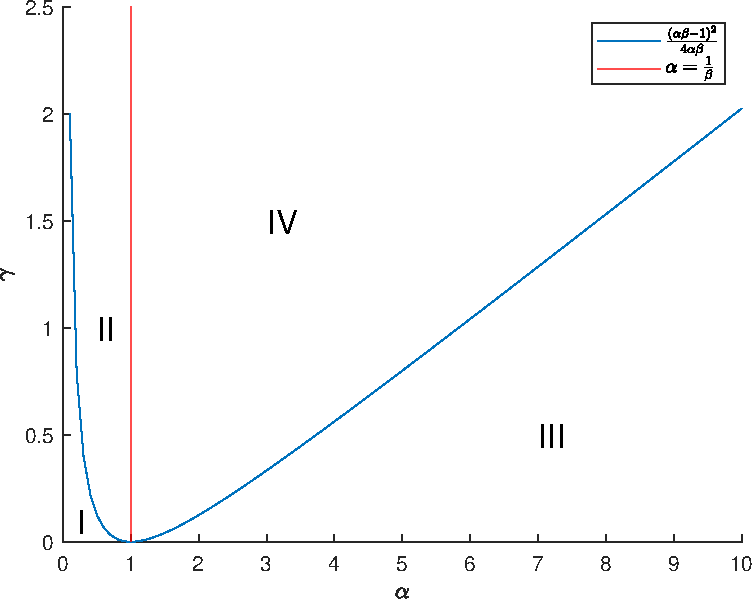
\includegraphics[scale = 1]{parameter_portrait.pdf}}
	\caption{Параметрический портрет системы (\ref{new_system}) при фиксированном значении параметра \( \beta = 1 \).}
\end{figure}


\newpage
Построим фазовые портреты системы в каждой из областей. Заметим, что у системы как и ожидалось может быть либо две либо четыре неподвижные точки.
\begin{figure}[h]
    \centering
    \subfloat[\centering Траектории системы в первой параметрической области.]{{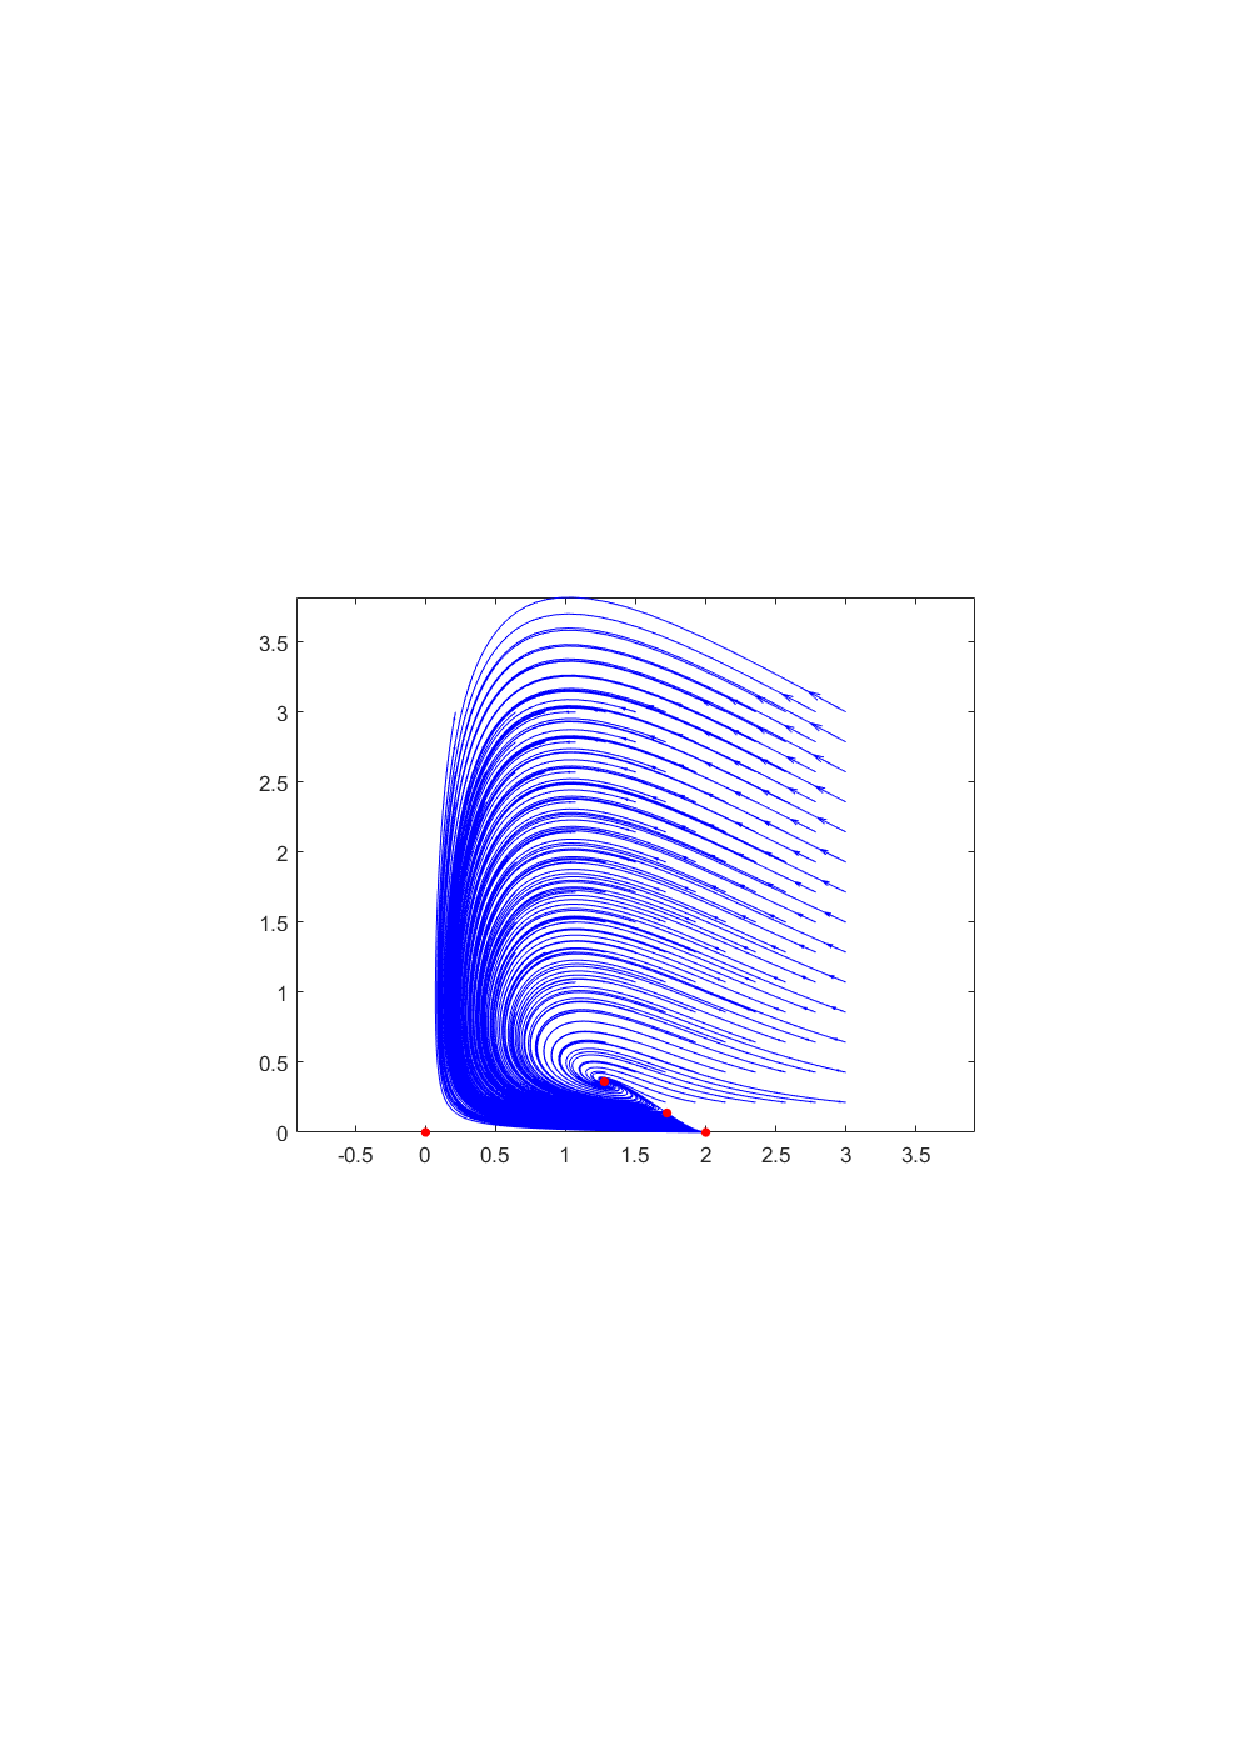
\includegraphics[width=7cm]{region_1.pdf} }}
    \qquad
    \subfloat[\centering Траектории системы во второй параметрической области.]{{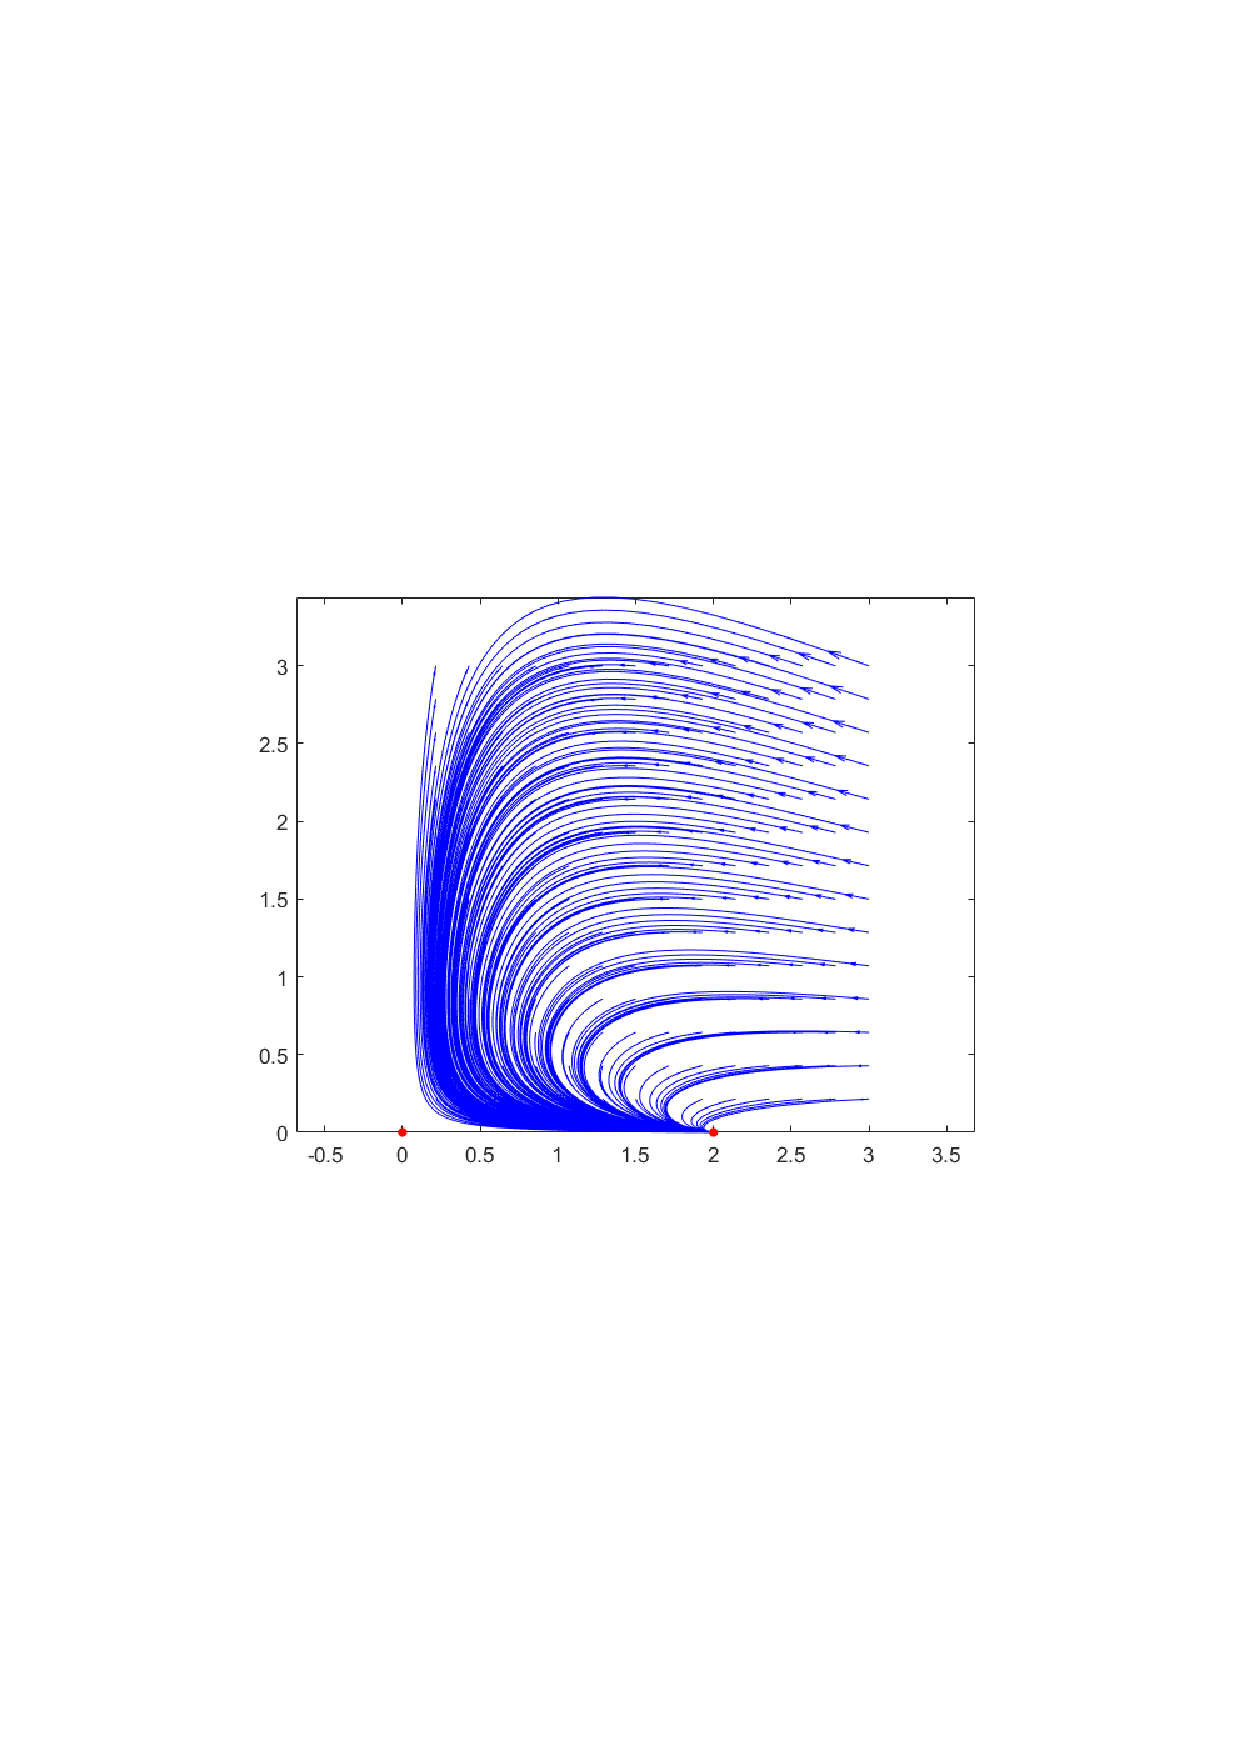
\includegraphics[width=7cm]{region_2.pdf} }}
    \\
    \subfloat[\centering Траектории системы в третьей параметрической области.]{{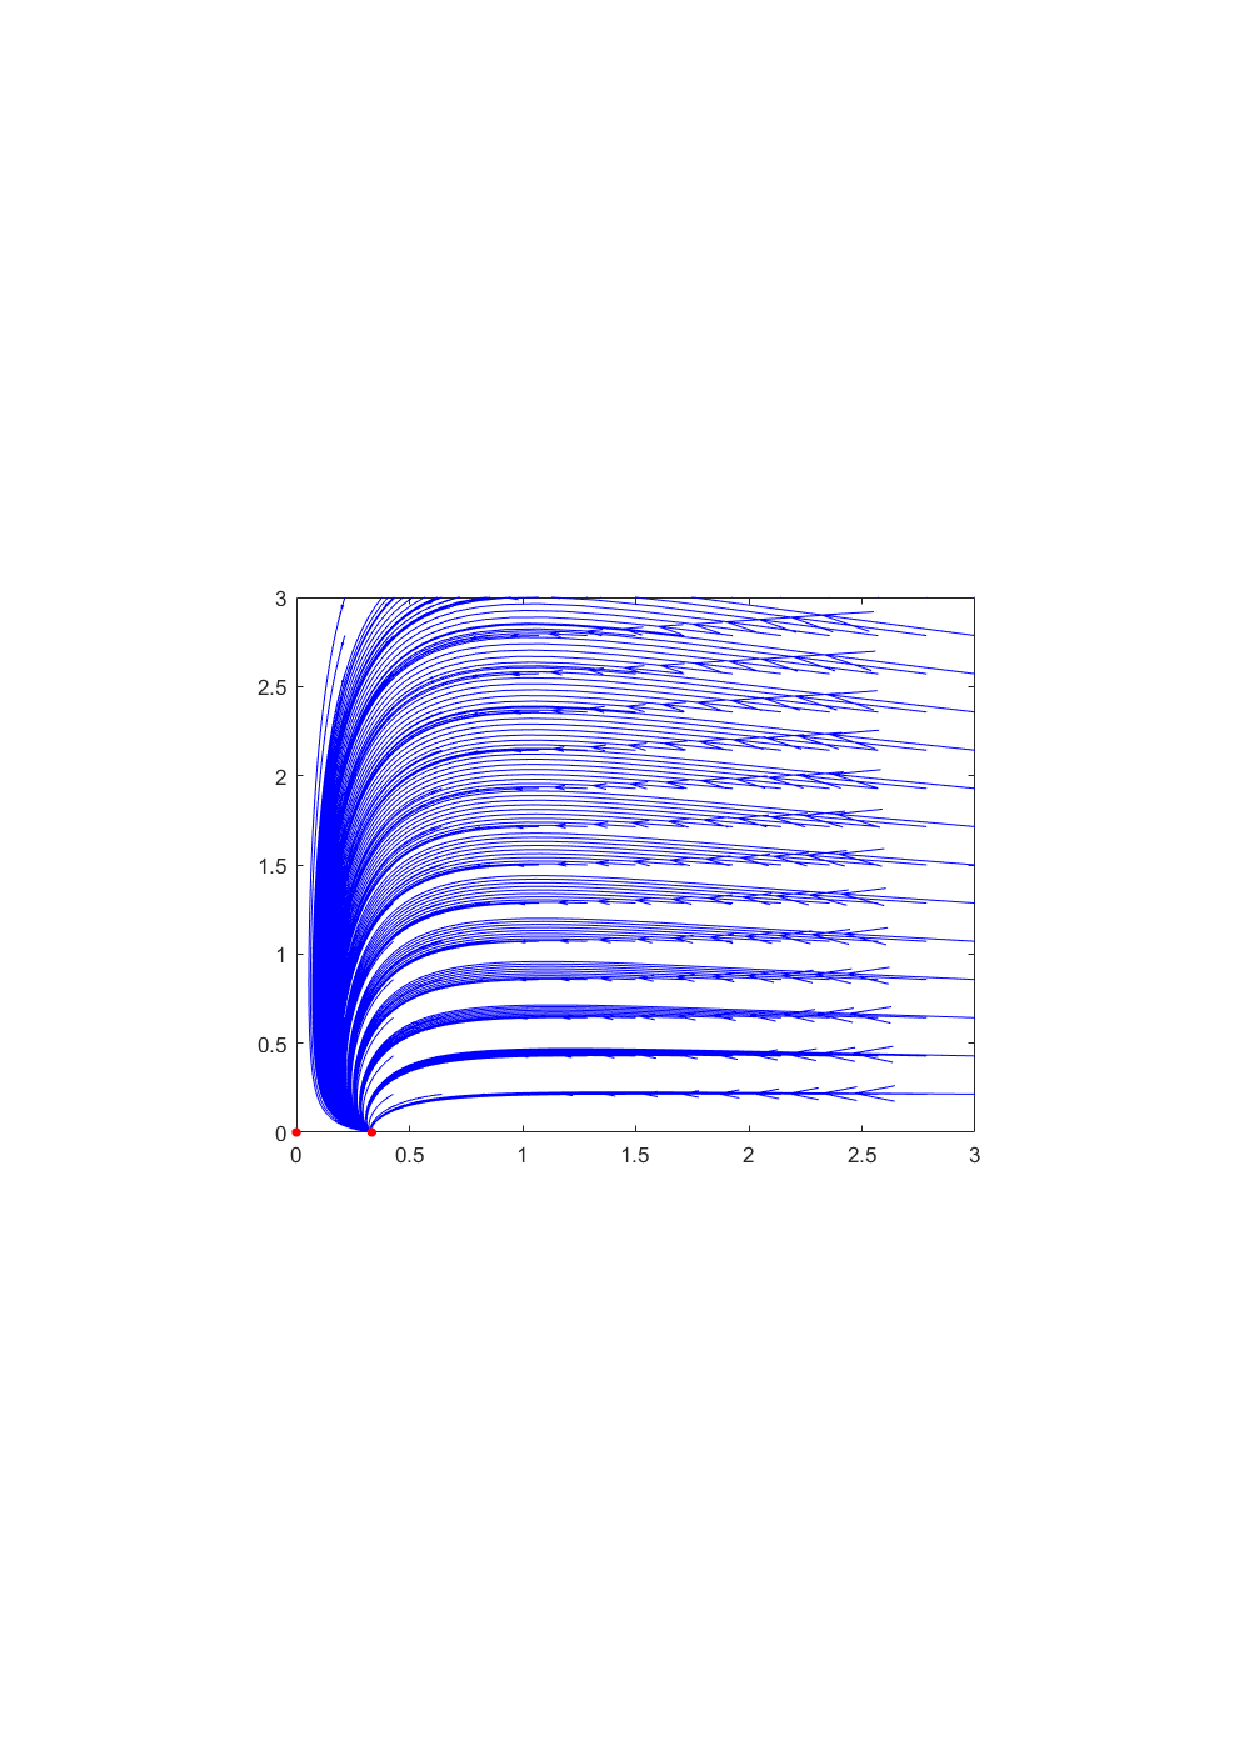
\includegraphics[width=7cm]{region_3.pdf} }}
    \qquad
    \subfloat[\centering Траектории системы в четвертой параметрической области.]{{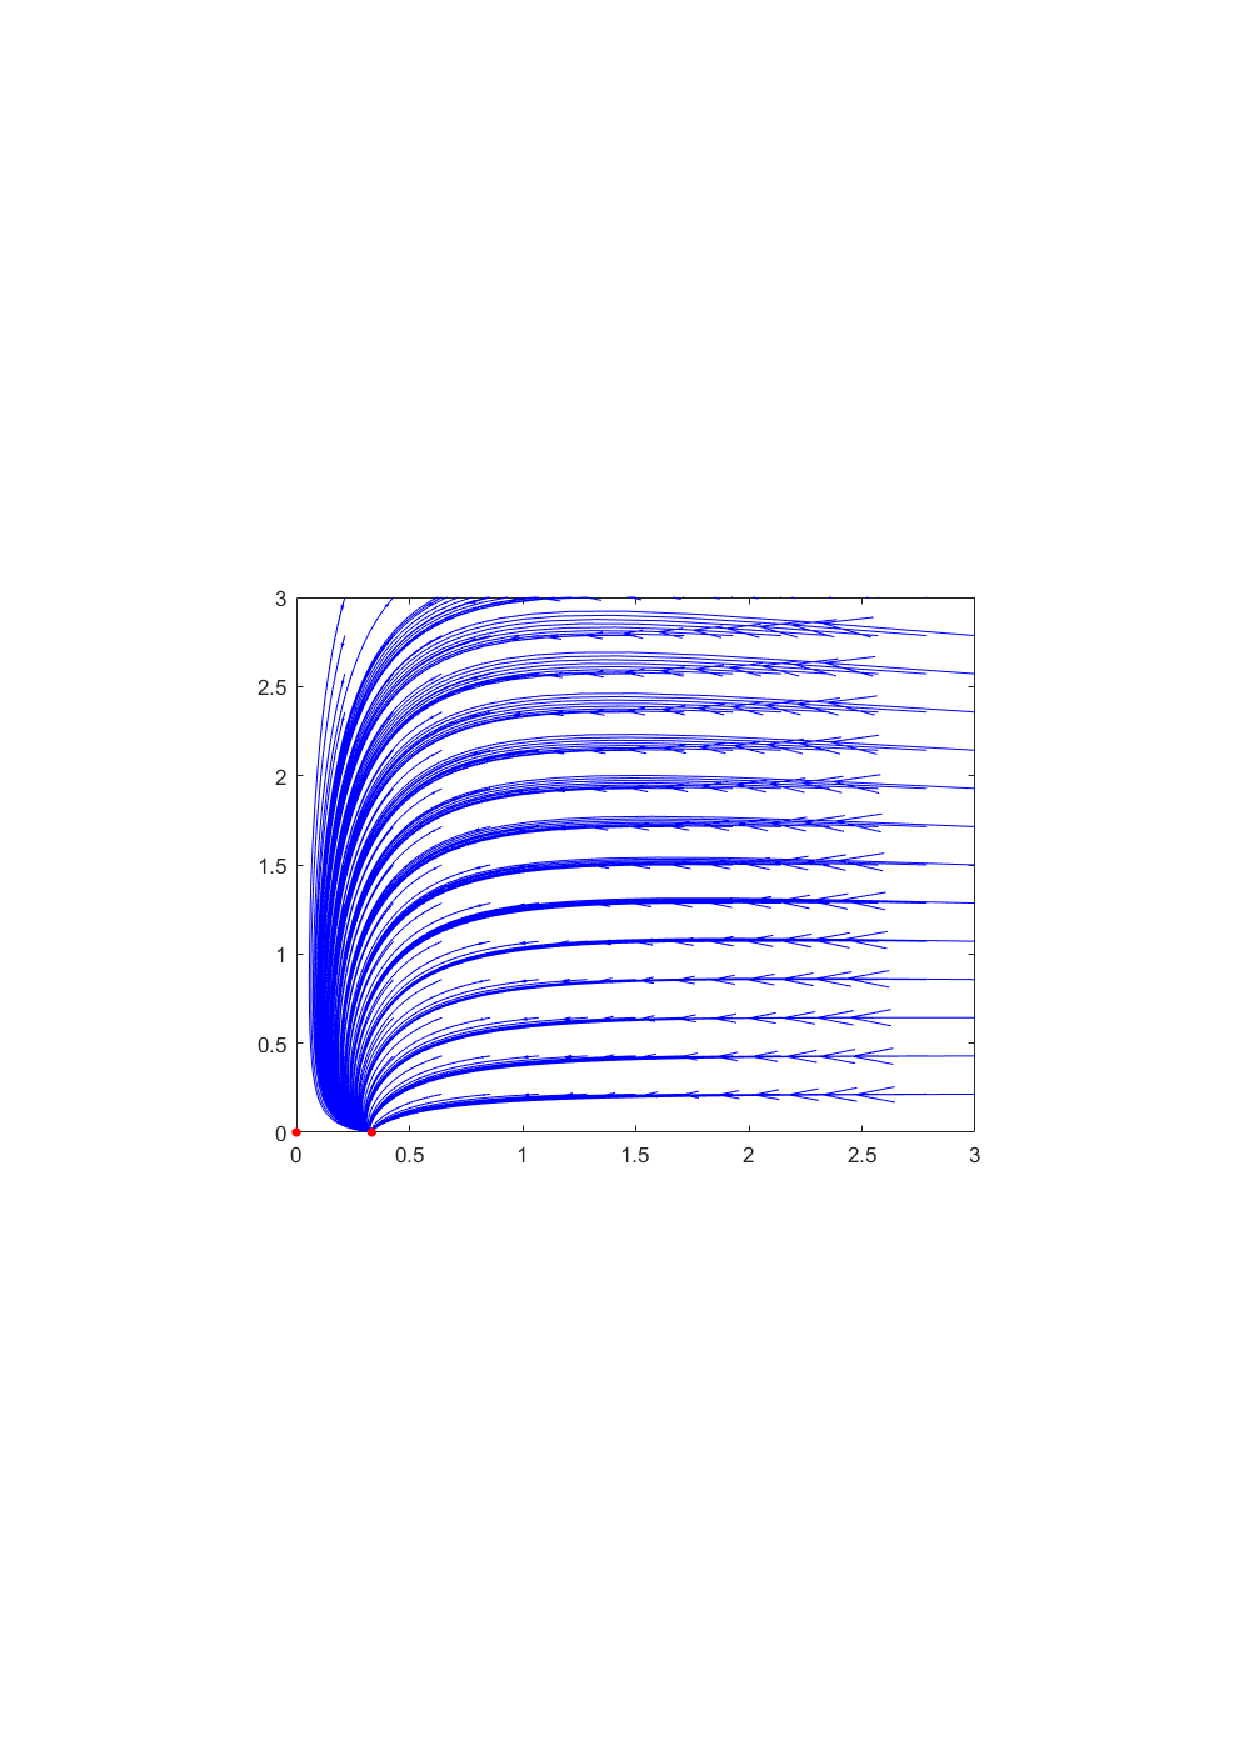
\includegraphics[width=7cm]{region_4.pdf} }}
\end{figure}

\newpage
\begin{figure}[h]
	\center{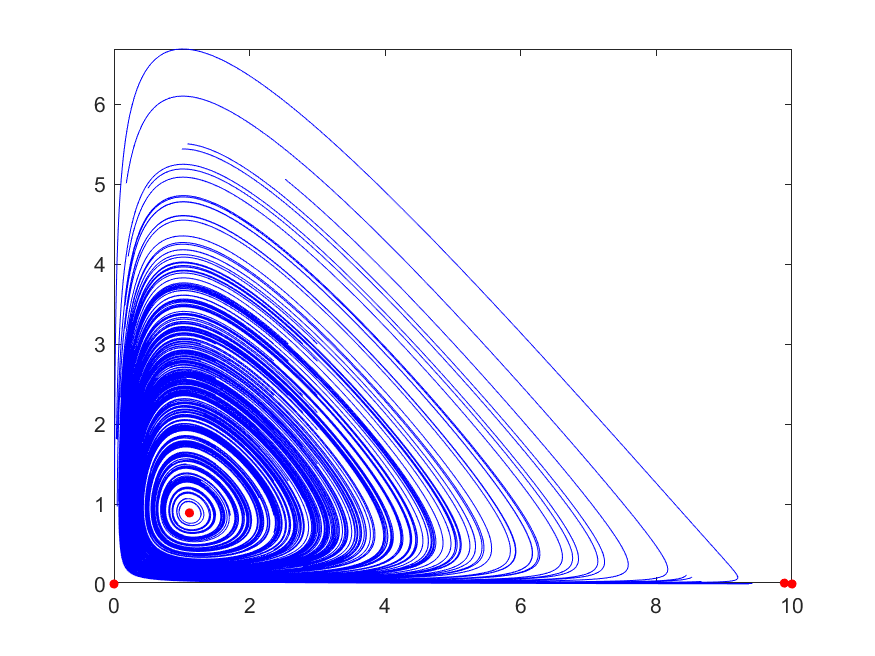
\includegraphics[scale = 1]{cicle.pdf}}
	\caption{Появление цикла около неподвижной точки \( u_3^* \). ( \( \beta = 1, \alpha = 0.1, \gamma  = 0.1 \) ).}
\end{figure}

\newpage
\begin{thebibliography}{0}
\addcontentsline{toc}{section}{Список литературы}
\bibitem{1}
Братусь А.\,С., Новожилов А.\,С., Платонов А.\,П. \emph{Динамические системы и модели биологии.} M.:Физматлит, 2011
\bibitem{2}
Базыкин А.\,Д. \emph{Нелинейная динамика взаимодействующих популяций.} М.: Институт компьютерных исследований, 2003
\end{thebibliography}
\end{document}